The ECal was installed in Hall B in the fall of 2014 and then calibrated using cosmic ray energy deposition in the crystals. The ECal was fully commissioned with a 2~GeV electron beam in December 2014 and demonstrated that the electronics read out chain from the ECal worked. The SVT was installed in the spring, and both detectors were calibrated using the data obtained from the 1.056~GeV electron beam in the 2015 engineering run. This chapter describes the methodology for calibration and the performance of the SVT and the ECal in the HPS experiment. 

\section{Silicon Vertex Tracker Performance}
The SVT measures particle hit locations on its silicon strips and reconstructs particle trajectories. The SVT momentum calibration strongly depends on the accuracy of its alignment in the magnetic field. In offline analysis, pairs of tracks are re-fit to obtain the vertex location. The invariant mass of the pair is reconstructed from the vertex of the two tracks by using the measured opening angle and the momenta. 

\subsection{Track reconstruction}

Hits in the SVT strips have an associated amplitude and time reported from the fit to the raw spectrum. These fitted hits are then clustered on the strips. The highest amplitude hit on the strip is designated as the ``seed" hit and must pass a threshold amplitude of $4\sigma_{noise}$. Hits on surrounding strips that are above $3\sigma_{noise}$ and within 8~ns of the seed time are added to the cluster. The position of the cluster is calculated using an amplitude-weighted position, and the time of the cluster is calculated as an amplitude-squared weighted time of the hits in the cluster~\cite{uemura_search_2016}. These are considered to be the 1D hits on the sensor. \\
\indent These 1D hits are converted into 3D hits by pairing the 1D hits with a cluster on the other sensor associated with that layer. These 1D hits are matched as coming from the same particle if they are close enough spatially such that the strips cross and if they are within 16~ns of each other. If they pass these cuts, then a 3D hit is created at their point of intersection. The 3D hit position is calculated from the track fit to these two hits because there is some small angle and distance between the two pair sensors.\\
\indent The initially constructed tracks are called seed tracks. Candidate seed tracks are first built by fitting a helix to hits in three SVT layers. These layers are considered to be the layers that ``seed" that track. The track is then extrapolated to a fourth layer which searches for a hit near the track that ``confirms" the track, and the track is re-fit to include this hit. If no hit is found, the track is discarded. Seed tracks that have been seeded and confirmed are then ``extended" to test for hits consistent with the track in the fifth and sixth layers. Only one hit layer is required to extend the track, but the track can match to hits in both layers. The designation of which specific layers are used for seeding, confirming, and extending tracks is the tracking strategy. During the 2015 engineering run, HPS used four different tracking strategies so that no track combination would be overlooked. Seed tracks that pass the strategy criteria are fit with a single helix to all the hits. The effects of multiple scattering are propagated with the position resolution at the downstream layers to reduce their importance in the fit.\\
\indent General Broken Lines (GBL) is a model that is used for the final track fitting that fully accounts for the effects of multiple scattering at each layer~\cite{blobel_fast_2011}~\cite{kleinwort_general_2012}. GBL treats each track as a series of track segments connected by scatters in each silicon sensor. A full GBL track fit is optimized to reduce the position residuals of each hit on the track and to minimize the kinks in scattering angles at each sensor on the track. Because each scatter is treated independently at each layer, scatters in downstream layers do not significantly alter the track trajectory upstream. GBL tracks are used for HPS analysis. 

\subsection{Momentum resolution}
The momentum resolution of the SVT is determined at the beam energy separately for the top and bottom by looking at tracks from elastically-scattered electrons. The momentum resolution of these tracks indicate the momentum resolution at the beam energy of 1.056~GeV. 

\begin{figure}[thb]
  \centering
      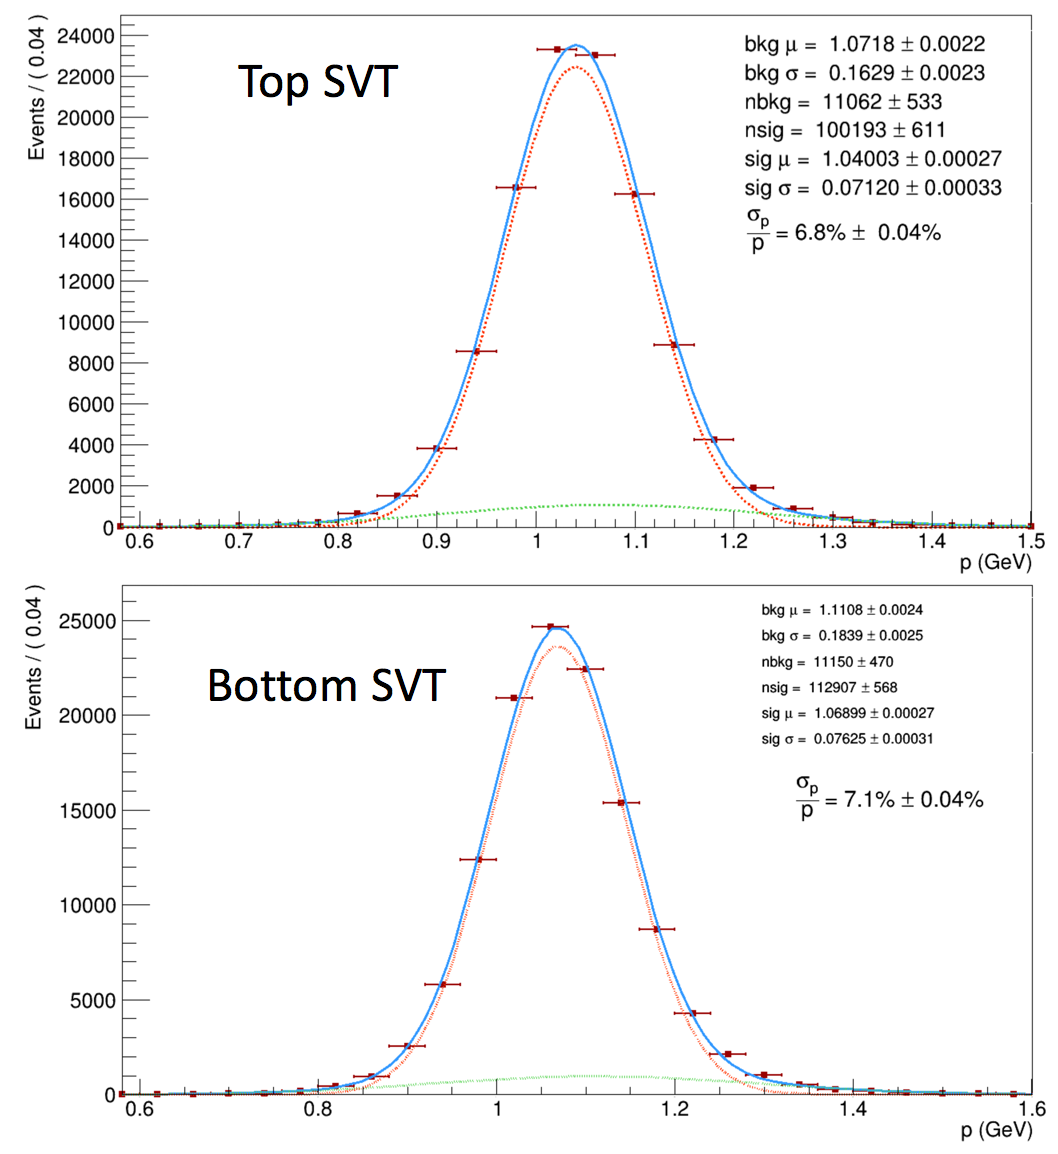
\includegraphics[width=0.75\textwidth]{pics/performance/SVTMom.png}
  \caption[Momentum resolution of the SVT]{The momentum resolution for elastically-scattered electron tracks passing through the top and bottom halves of the halves of the ECal separately. The momentum resolution is approximately 7$\%$~\cite{moreno_search_2016}.}
  \label{Figure:pRes}
\end{figure}

By using the measured ECal energy and resolution (see discussion in section~\ref{EcalResData}), one can also extract the momentum resolution of the SVT for different track momenta. By looking at tracks matched to clusters in the ECal and fitting the ratio of the measured ECal energy $E$ to the SVT momentum $P$ distribution, the momentum resolution is extracted as
\begin{equation}
	\label{eq:pres}
	\sigma_P = P\sqrt{\sigma_{E/P}^2-\Big(\dfrac{\sigma_E}{E}\Big)^2} 
\end{equation}
where $\sigma_{E/P}$ is the measured width of the $E/P$ distribution fit with a Gaussian, and $\sigma_E/E$ is the energy-dependent ECal energy resolution. The SVT momentum resolution is roughly 7$\%$ across the range of momenta accessible in the 2015 run configuration (see Figure~\ref{Figure:pResExtrap}). The momentum resolution is within 0.5$\%$ of the resolution found by fitting the SVT elastically-scattered electron tracks shown in Figure~\ref{Figure:pRes}.

\begin{figure}[thb]
  \centering
      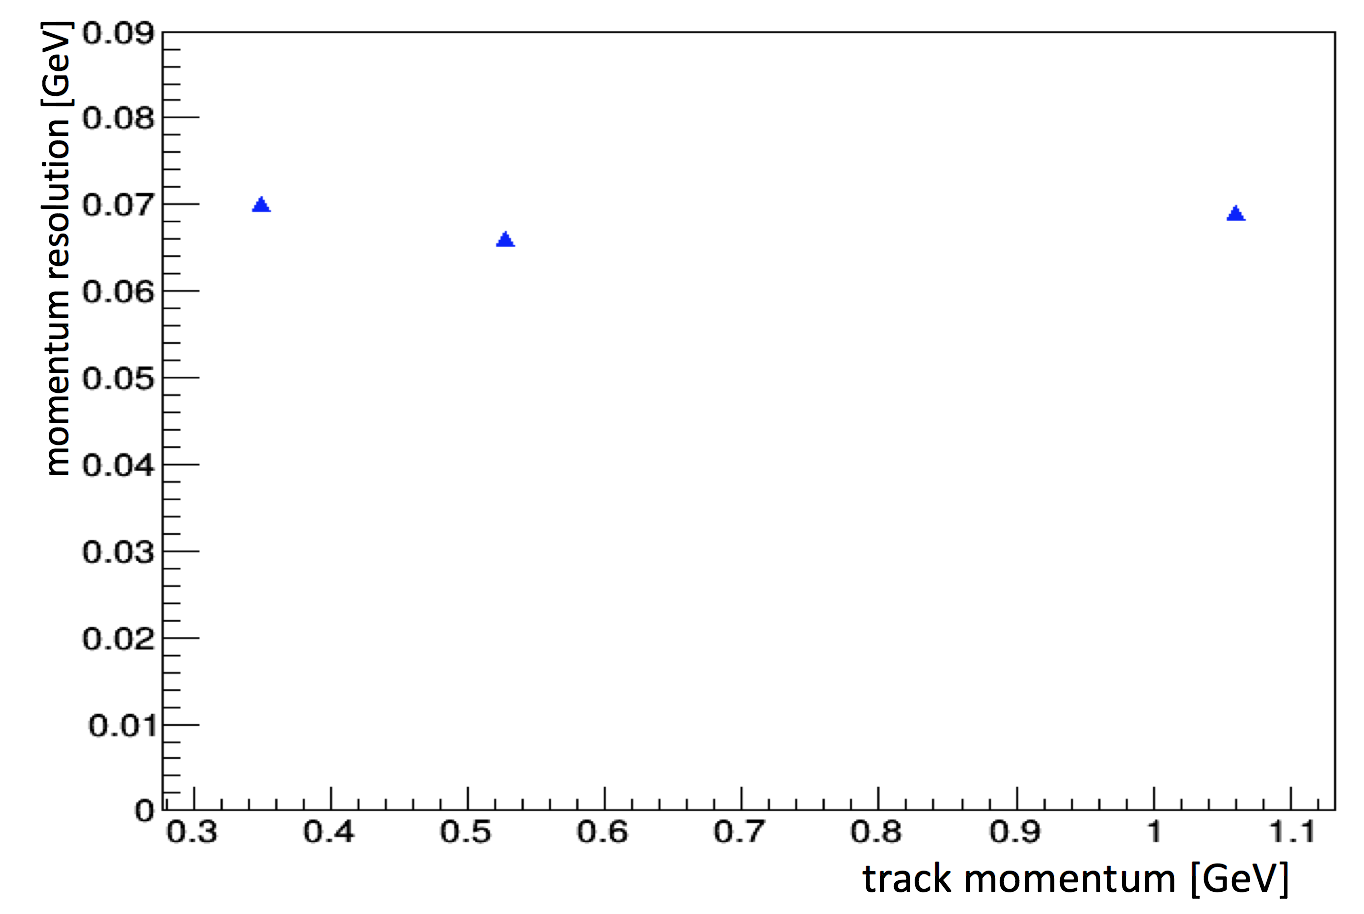
\includegraphics[width=0.75\textwidth]{pics/performance/pResExtrapolated.png}
  \caption[Momentum resolution of the SVT extracted from $E/P$]{The momentum resolution of the SVT is roughly constant for all accessibly momenta at 7$\%$. This is roughly consistent with the momentum found in Figure~\ref{Figure:pRes}.}
  \label{Figure:pResExtrap}
\end{figure}

\subsection{Tracking efficiency}

Reconstructed GBL tracks require a minimum of five hit tracks but can have six hit tracks. The tracking efficiency per SVT layer is extracted from the ratio of six-hit tracks to the number of five or more hit tracks missing a certain layer. It is better than 98$\%$ for layers 2--5. Layer 1 has the lowest efficiency of all the tracking layers at around 90$\%$ as shown in Figure~\ref{Figure:trackEff}. The inefficiency of Layer 1 is thought to be due to the high rates from being close to the active beam. 

\begin{figure}[thb]
  \centering
      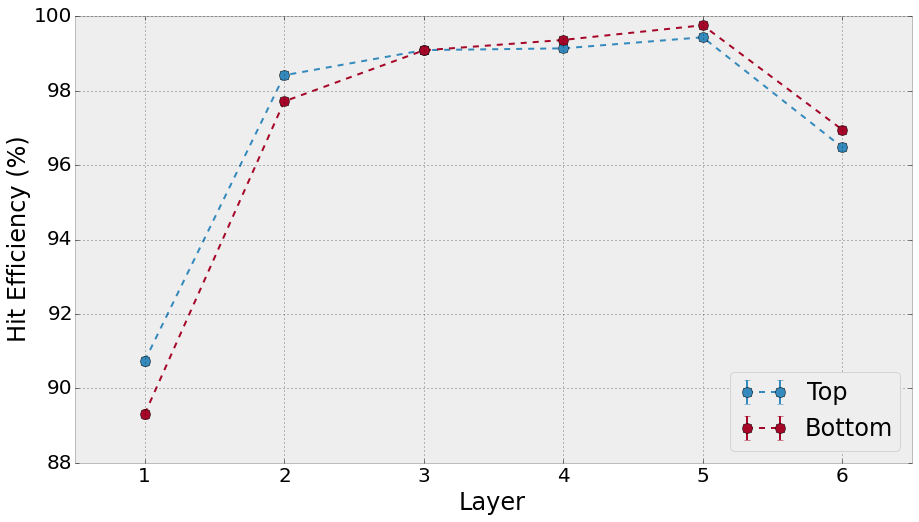
\includegraphics[width=0.75\textwidth]{pics/performance/engrun2015_hit_efficiency_vs_layer.png}
  \caption[Tracking efficiency of the SVT by layer]{The tracking efficiency is shown by layer as a comparison between the number of six-hit tracks and the number five or more hit tracks missing a particlular layer. The tracking efficiency is generally high (better than 95$\%$), but Layer 1 is lower than the other layers at  90$\%$~\cite{moreno_search_2016}.}
  \label{Figure:trackEff}
\end{figure}

\subsubsection{Tracking efficiency using three particle events}
We can also measure the overall tracking efficiency of the SVT by using three particle final state events. These may result from tridents or wide angle bremsstrahlung pair conversion. These events require three clusters in the ECal and two or more tracks. The three clusters are chosen to ensure that they come from events with three particles. For any two SVT tracks, the third track must have a projected momentum that would have passed through the SVT. For events with three tracks, the momentum sum (as shown in Figure~\ref{Figure:psumtrks}) reflects the quality of the selection criteria. 
\begin{figure}[thb]
  \centering
      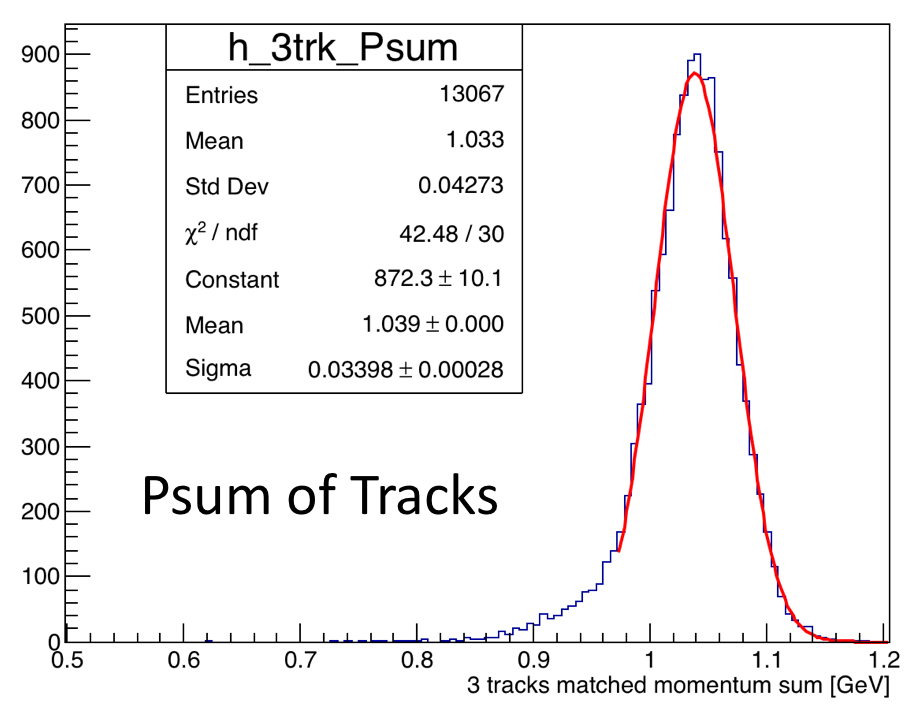
\includegraphics[width=0.55\textwidth]{pics/performance/pSum_3trk.png}
  \caption[Momentum sum of three track final state particles]{The momentum sum of three track final state particles is shown.}
  \label{Figure:psumtrks}
\end{figure}

The combined cluster energy sum was required to be within 10$\%$ of the beam energy so as to eliminate events that did not contain three particles. The ratio of the number of three track events to the number of two or more track events tells us the efficiency of measuring a certain particle. This technique is limited to measuring the efficiency at low momentum ($<0.5$~GeV/c).\\
\indent There are three different topologies considered for each particle type ($e^+$ or $e^-$): whether it was in a half (top or bottom) by itself, in the half with the electron that is closest to the beamline, or in the half with the electron that is farthest from the beamline. The efficiencies for these topologies were found to be the same for particles in the top versus the bottom so those results were combined to improve statistics. Bins with low statistics were thrown out. The efficiencies can be seen in Figure~\ref{fig:eff3prong}.


\begin{figure}[hbt]
%\begin{center}
\begin{minipage}{0.55\textwidth}
	  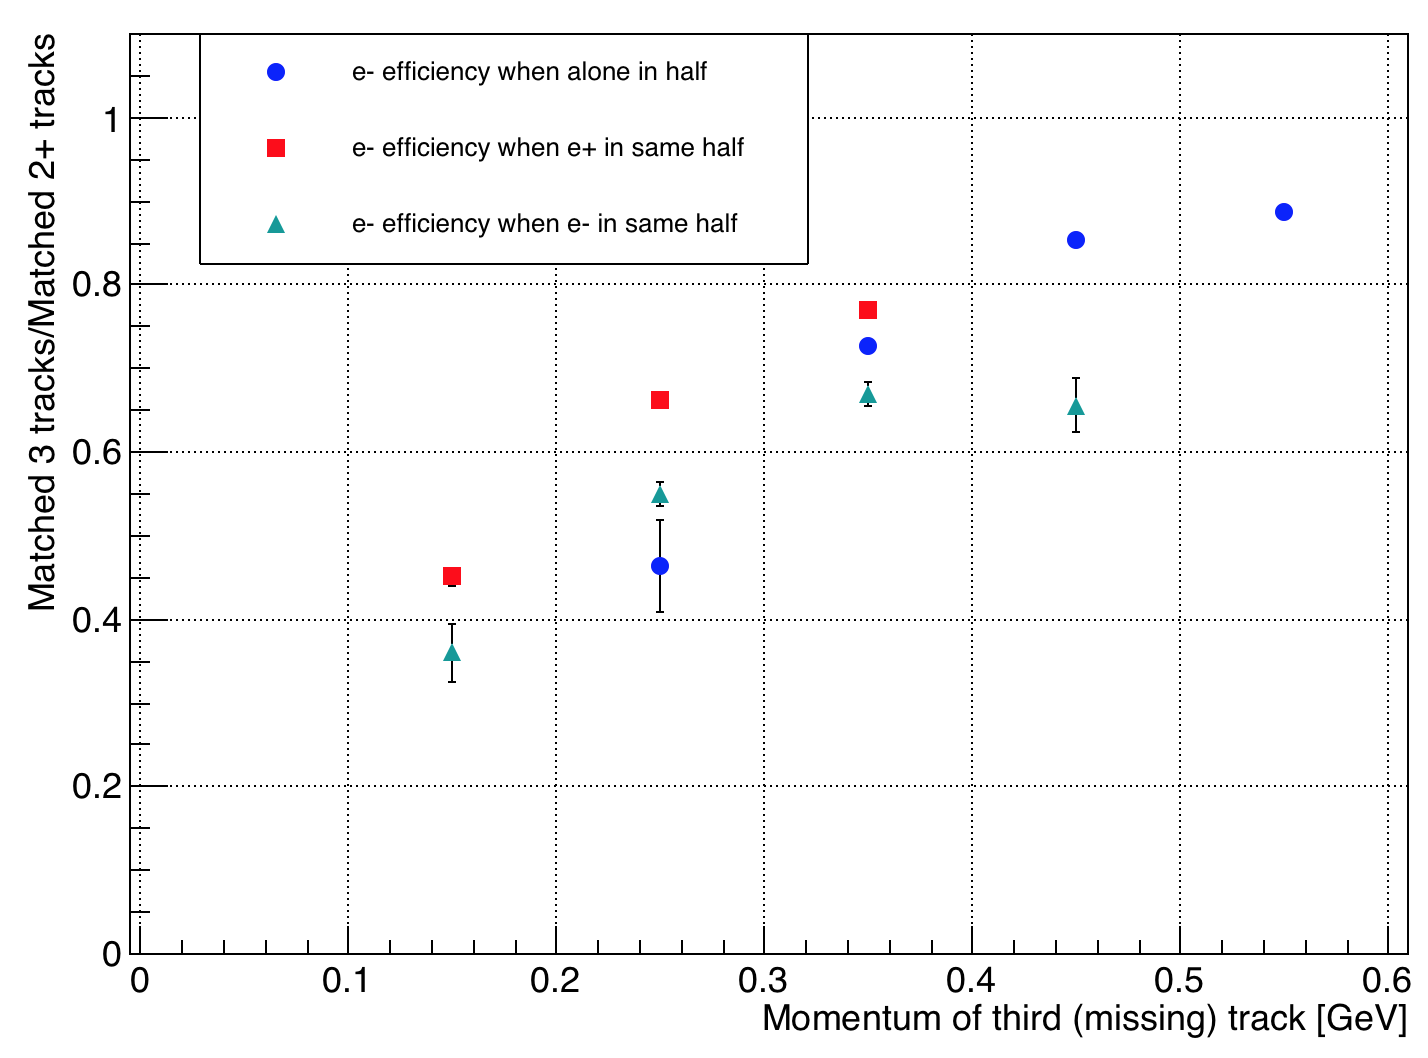
\includegraphics[width=\textwidth]{pics/performance/em_trkEff.png}
    	  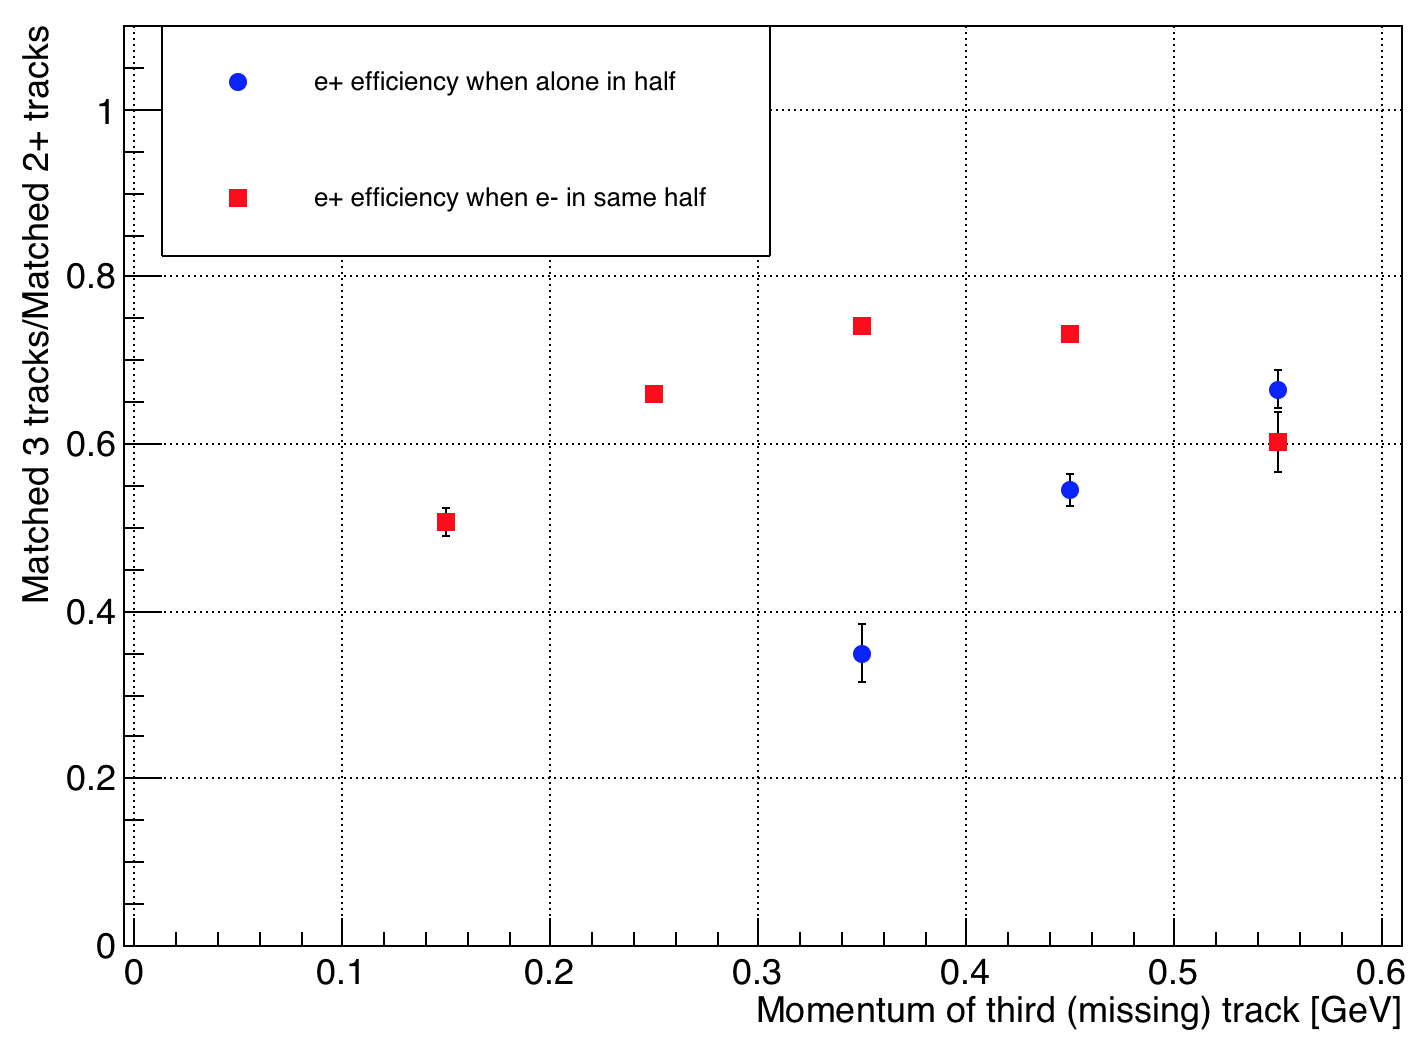
\includegraphics[width=\textwidth]{pics/performance/ep_trkEff.png}
%\end{center}
\end{minipage}\hfill\begin{minipage}{0.32\textwidth}
\caption[Tracking efficiency from three particle final state events]{ \label{fig:eff3prong} \baselineskip 11pt
{The efficiency for tracking a particle as a function of its momentum. The tracking efficiency for electrons (top) and positrons (bottom) is shown separately for different topologies.}
}
\end{minipage}
\end{figure}

The resulting electron efficiency increases with momentum and plateaus around 400~MeV. This turn on of the efficiency was not previously seen in the trident Monte Carlo. The positron efficiency is more difficult to interpret and has yet to be fully understood. The positron spectrum may be more influenced by the pair-converted wide angle bremsstrahlung. The general tracking efficiency assumed in the proposal was 0.85. 

%%%%%%%%%%%%%%%%%%%%%%%%%%%%%%%%%%%%%%%%%%%%%%%%%%%
\section{Electromagnetic Calorimeter}
The ECal was calibrated both in energy and time. The first calibration performed before receiving beam from the accelerator was the cosmic ray energy calibration. A full timing calibration of the ECal was performed using the accelerator RF signal and cluster-pair events. A final calibration using physics events from elastically-scattered beam energy electrons and events from wide angle bremsstrahlung (WAB) yielded the full calibration of the ECal for all energies.  

\subsection{Energy Reconstruction}
The ECal uses an adapted version of the clustering algorithm that was used by the CLAS IC. The geometrical arrangement of the crystals differs greatly from that used by the IC and required detailed studies and simulations to reconstruct the incident particle energy. The angles of incidence of the particles (electrons, positrons, and photons) entering the ECal varies significantly across the ECal. The edge effects in the ECal are substantial due to the horizontal split between the top and bottom halves and  the proximity to the beam. \\
\indent As a particle enters the ECal, it deposits all of its energy in the crystal material. Due to the segmentation of the calorimeter, multiple adjacent crystals will each contain different fractions of the incident particle's energy. In offline clustering, the energy is reconstructed by summing all of the modules that measured some amount of the incident particle energy. The total reconstructed energy is always proportional to and less than the incident particle energy due to energy loss effects. These energy loss effects can best be studied through simulation and experimental testing with the electronics.\\
\indent Clustering searches for a crystal having energy higher than all the immediately adjacent modules. This module becomes the ``seed" hit and initializes the cluster. The clustering algorithm then searches for hits surrounding the seed hit with lower energy and adds these hits to the cluster.The process continues by searching for hits surrounding the clustered hits with lower energy to add to the cluster. When two clusters overlap such that it is difficult to identify which hit a cluster belongs to, the energy of that module is divided between the two clusters in proportion to the seed hit energies of the two clusters.  Once all hits have been clustered, the cluster energy is the summed energy of all of the hit contributions within the cluster. 

\subsubsection{Simulations}
Simulations were performed using the fully modeled detector geometry in SLIC as part of the standard HPS software package. The geometry includes all strips of the SVT, vacuum chambers, ECal crystals, and relevant dead material. The software also tracks particles through a 3D magnetic field map corresponding to the field values for 1~GeV beam running~\cite{szumila-vance_hps_2016}.\\
\indent Single electrons, positrons, and photons were simulated at discrete energies of 0.2, 0.3, 0.4, 0.5, 0.6, 0.7, 0.8,  0.9, 1.0, and 1.1~GeV to uniformly cover the range of energies detectable in the 2015 engineering run. The simulation uses the full reconstruction chain excluding pile-up effects. Offline reconstruction clusters all of the adjacent ECal crystals containing some fraction of the incident particle energy so that the total cluster energy can be measured as the sum of the energy carried by all of the crystals in a cluster. The offline cluster reconstruction uses the same thresholds used in data and production Monte Carlo: 7.5~MeV for individual hits, 50~MeV for seed hits in clusters, and 100~MeV for cluster energies.\\
\indent Due to the complex showering cascade that occurs when a particle deposits its energy in the ECal, several adjacent crystal modules contain some fraction of the incident energy of the particle. These modules are clustered in offline reconstruction to obtain the total deposited energy of the incident particle. The reconstructed energy, $E_{rec}$, not corrected for shower loss effects is 

\begin{equation}
\label{eq:eclsum}
E_{rec} = \sum_i E_i    
\end{equation}
where $E_i$ is the energy of the $i^{\textrm{th}}$ module in the cluster. Some energy is lost between crystals and out the back of the ECal. After summing the ECal energy over the cluster, the incident particle energy can be found by correcting for the shower loss effects as  

\begin{equation}
\label{eq:eclsf}
E_{corr} = \dfrac{E_{rec}}{f}   
\end{equation}
where $f$ is the energy-dependent ratio of measured to incident particle energy. This factor is obtained from simulation. The energy loss corrections as derived from Monte Carlo are shown in Figure~\ref{Figure:ecorr}.

\begin{figure}[thb]
  \centering
      \includegraphics[width=0.75\textwidth]{pics/performance/energycorrection.pdf}
  \caption[ECal energy shower correction functions derived from simulation]{The fraction $f$ is the reconstructed cluster energy, $E_{rec}$, divided by the Monte Carlo generated particle energy, $E_{gen}$, and is plotted versus the reconstructed energy. Each simulated particle type is shown in a different color, and the functional fit of Equation~\eqref{eq:ecorrfunc} for each particle is shown by the dashed lines.}
  \label{Figure:ecorr}
\end{figure}

The difference in the energy corrections for the various particle types arises from geometrical effects and the incident angles of the particles entering the crystals~\cite{szumila-vance_hps_ecal_2014}. The focal point of the calorimeter, the point toward which all crystals are angled, lies 80~cm from the front face of the ECal. The HPS target is beyond this focal distance at approximately 1.4~m from the face of the ECal and is offset beam right in the pair spectrometer magnetic field. Charged particles produced at the target take different trajectories from the target to the ECal due to the magnetic field. This affects the entry angle of the particle into a crystal and requires a charge and momentum-dependent correction. The form of the energy correction function for the central region of the ECal is described by a three parameter fit:\\

\begin{equation}
	\label{eq:ecorrfunc}
	\dfrac{E_{rec}}{E_{gen}} = \dfrac{A}{E_{rec}}+\dfrac{B}{\sqrt{E_{rec}}}+C 
\end{equation}

The shower leakage effects in crystals becomes significant close to the calorimeter edge. The energy reconstruction deteriorates rapidly in the crystals closest to the edge but is relatively constant in central region of the ECal. The energy reconstruction at the edges was characterized using Monte Carlo as a function of particle hit position in the ECal relative to the inner beam gap edge. In Equation ~\eqref{eq:ecorrfunc}, parameter $A$ is not strongly correlated with position and remains constant for a given particle type. Parameters $B$ and $C$  strongly depend on the cluster position relative to the beam gap edge of the ECal. These dependencies can be seen for electrons in Figure~\ref{Figure:sfparEdge}.

\begin{figure}[htb]
  \centering
      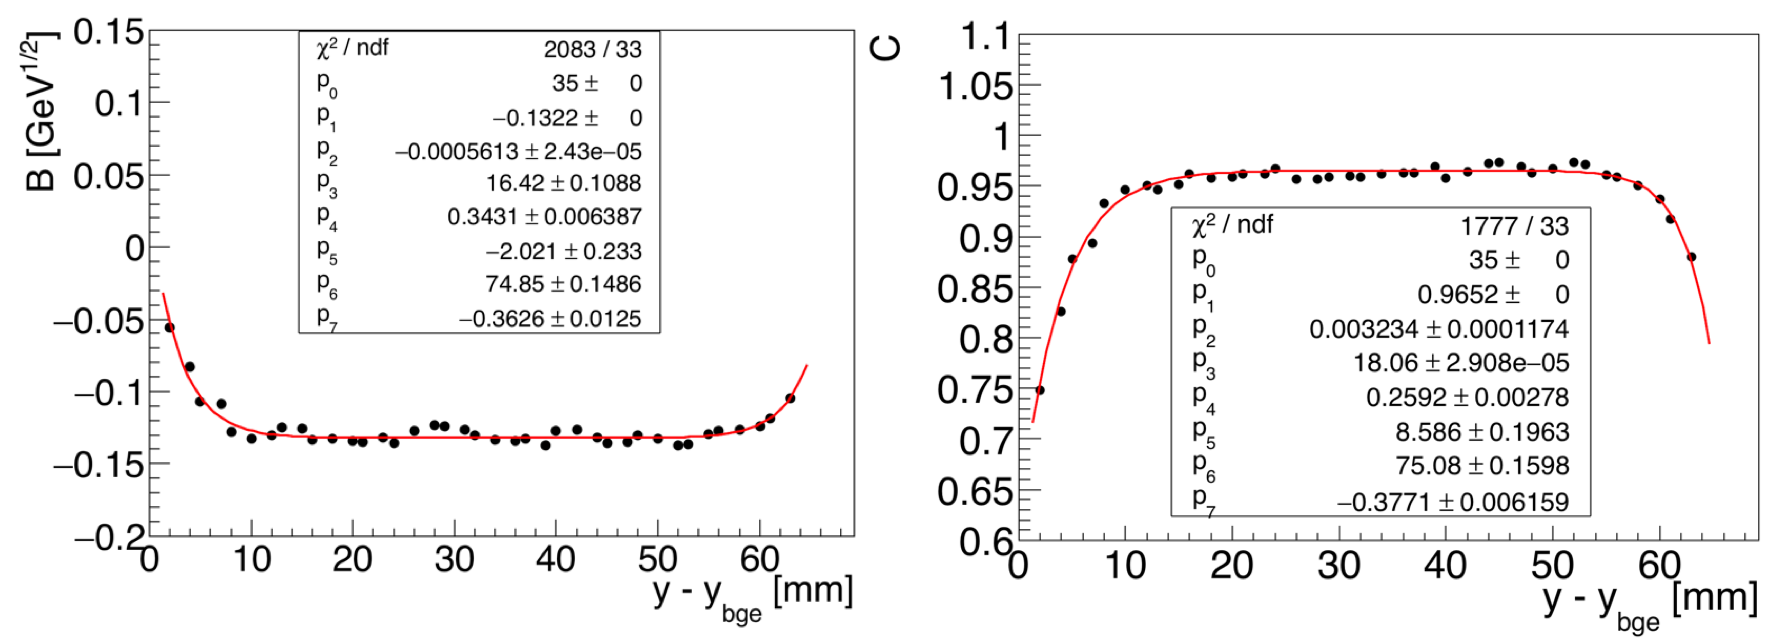
\includegraphics[width=1.0\textwidth]{pics/performance/sfparEdgeFit.png}
  \caption[ECal energy shower parameters for electrons relative to the inside beam gap edge]{Parameters $B$ and $C$ from Eq.~\ref{eq:ecorrfunc} for electrons, as a function of vertical position
relative to the innermost beam gap edge.}
  \label{Figure:sfparEdge}
\end{figure}
The energy leakage parameters $B$ and $C$ can be fit with two functions at the edges that match in the central region of the ECal, away from the edges of the calorimeter. The equations used to fit the $B$ and $C$ parameters are described by:

\begin{equation}
\begin{split}
\label{eq:p1parlt}
B(y<p_0) = p_1-p_2 e^{-(y-p_3)p_4}\\
B(y>p_0) = p_1-p_5 e^{-(y-p_6)p_7}
\end{split}
\end{equation}

\begin{equation}
\begin{split}
\label{eq:p2parlt}
C(y<p_0) = p_1-p_2 e^{-(y-p_3)p_4}\\
C(y>p_0) = p_1-p_5 e^{-(y-p_6)p_7}
\end{split}
\end{equation}

The energy leakage correction functions are relatively constant in the central region of the calorimeter and are matched at a central distance $p_0$. For columns containing 5 crystals, the distance to the beam gap edge is the absolute value of the distance from the cluster centroid to the innermost beam gap edge. In the regions above and below the region where row 1 crystals are removed in the ECal, additional consideration is made when calculating the distance to the inner beam gap edge in order to be consistent with other regions of the ECal. At distances within 35~mm to the inner beam gap edge of row 2 when above and below the electron hole, the distance to the inner beam gap edge for the corrections corresponds to the inner edge of the row 2 crystals. At distances greater than 35~mm from the inner beam gap edge above and below the electron hole, the correction is applied relative to the inner beam gap edge distance as calculated to the inner edge of the row 1 crystals. This ensures that the edge corrections are consistent throughout the different regions of the ECal. For completeness, the corresponding energy correction parameters for positrons and photons are seen in Figures~\ref{Figure:sfparEdgeEP} and \ref{Figure:sfparEdgeP}, respectively. 

\begin{figure}[htb]
  \centering
      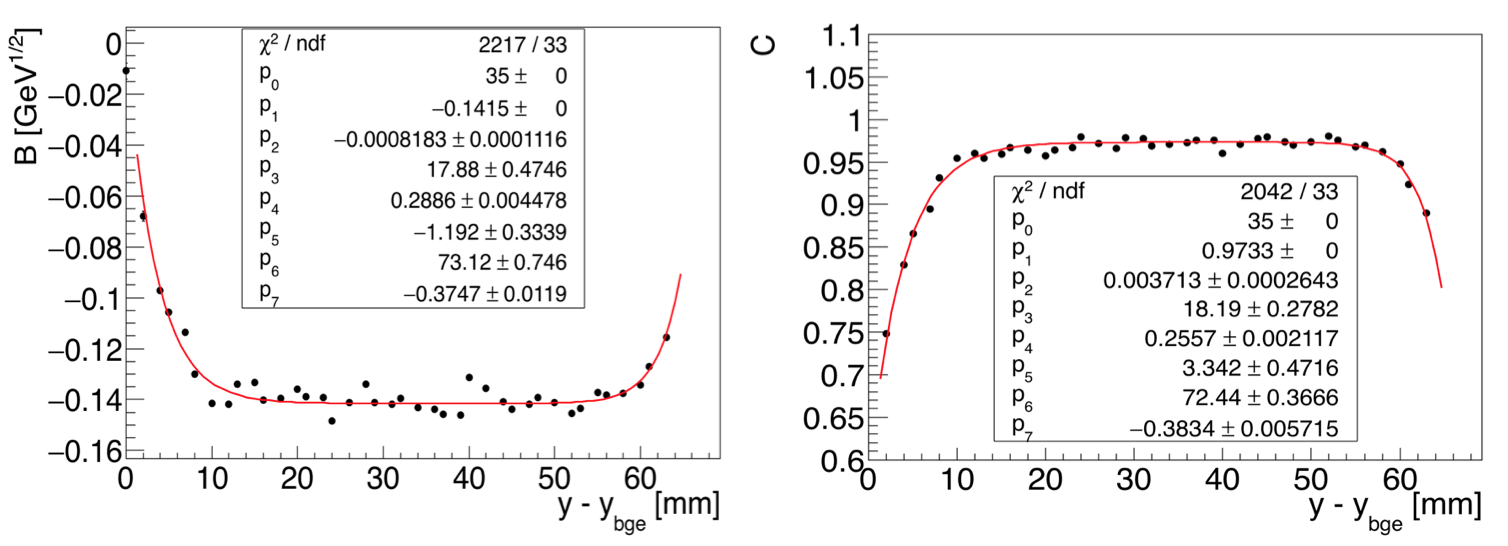
\includegraphics[width=1.0\textwidth]{pics/performance/sfparEdge_ep.png}
  \caption[ECal energy shower parameters for positrons relative to the inside beam gap edge]{Parameters $B$ and $C$ from Eq.~\ref{eq:ecorrfunc} for positrons, as a function of vertical distance from the innermost beam gap edge.}
  \label{Figure:sfparEdgeEP}
\end{figure}

\begin{figure}[htb]
  \centering
      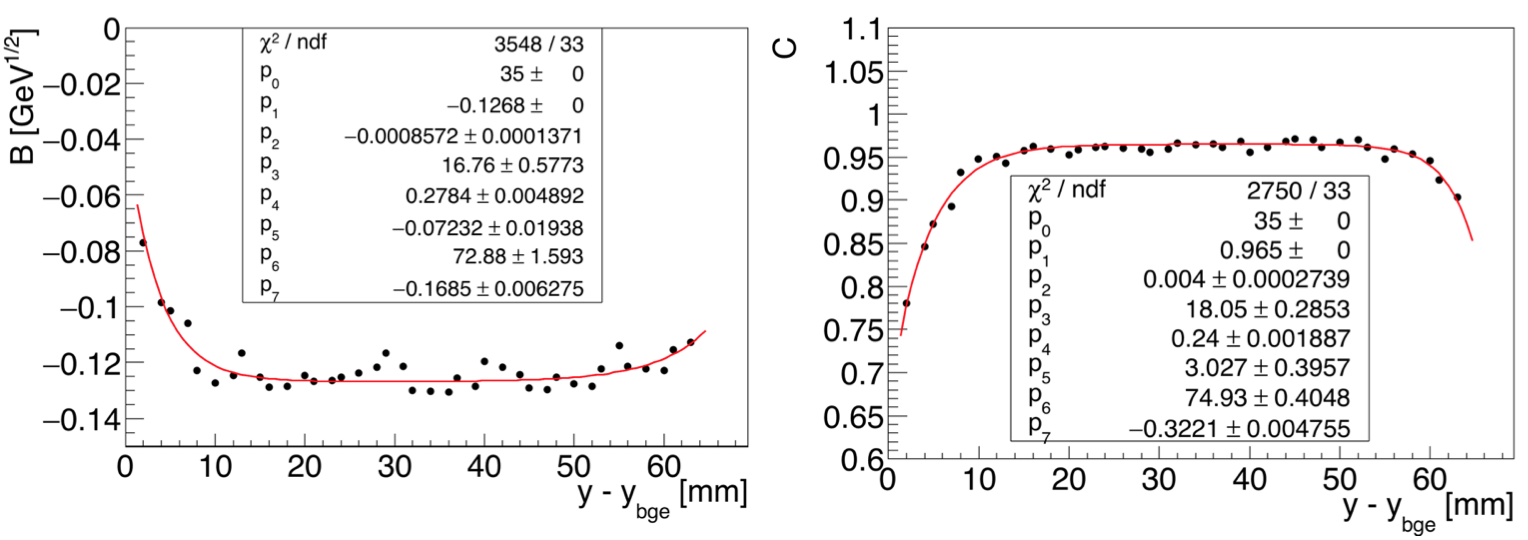
\includegraphics[width=1.0\textwidth]{pics/performance/sfparEdge_p.png}
  \caption[ECal energy shower parameters for photons relative to the inside beam gap edge]{Parameters $B$ and $C$ from Eq.~\ref{eq:ecorrfunc} for photons, as a function of vertical position
relative to the innermost beam gap edge.}
  \label{Figure:sfparEdgeP}
\end{figure}

The energy correction fraction is relatively constant beginning at approximately 1~cm from the ECal edges. As a result, we define the fiducial region of the ECal to be more than 1~cm from the edge, or approximately 3/4 of the front face crystal dimension. This result is consistent with the findings for the CLAS IC~\cite{szumila-vance_hps_ecal_2014}.\\
\indent In reconstruction of the data, the energy of all the crystals in the cluster are summed to make the uncorrected, reconstructed cluster energy. Separately, tracks from the SVT are matched with clusters in the ECal. From the curvature of the track, the particle type can be determined as being either a positron or electron. Clusters that have no matching track are determined to be due to photons. The position of the track at the ECal and the particle type are used to apply the corrections in Equation~\eqref{eq:ecorrfunc} that contain the further edge corrections (if necessary) from Equations~\eqref{eq:p1parlt} and~\eqref{eq:p2parlt}. Photon clusters are corrected using the photon-type energy and position corrections to the cluster in the ECal.  

\subsubsection{Energy resolution}

The energy resolution of the ECal is energy-dependent and improves with energy as approximately $1/\sqrt{E}$. 
\begin{figure}[htb]
  \centering
      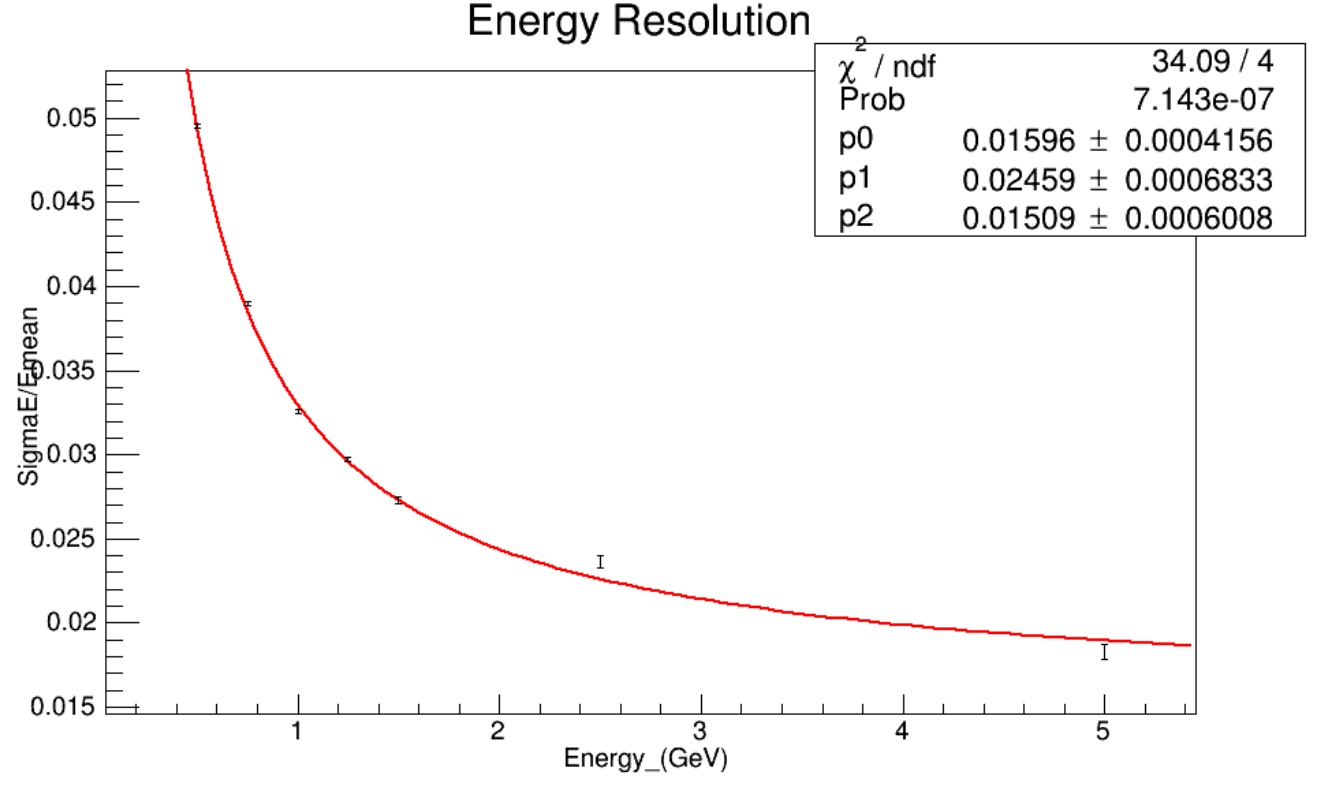
\includegraphics[width=0.6\textwidth]{pics/performance/eResFitMC.png}
  \caption[ECal fractional energy resolution fitted from simulation]{ECal fractional energy resolution from simulation. The points show the fractional energy resolution extracted from simulation, and the red line is the fit to the points.}
  \label{Figure:eResFitMC}
\end{figure}
From simulation, we obtain the energy resolution as shown in Figure~\ref{Figure:eResFitMC}. The fit shown in Figure~\ref{Figure:eResFitMC} is described by
\begin{equation}
\label{eq:eResMC}
\dfrac{\sigma_E}{E} (\%) = \dfrac{1.60}{E} \oplus \dfrac{2.46}{\sqrt{E}} \oplus 1.51
\end{equation}
where the energy is in units of GeV. The first term corresponds to the preamplifier noise. We were expecting 3~MeV$\times \sqrt{10} = 0.009$~GeV, where 10 is the average number of hit crystals, but we instead measured 0.016~GeV. Simulation does not include the FADC error (expected to be 1.3~MeV~\cite{charles_2014}) which contributes a term (in $\%$) as $0.13\sqrt{10}\textrm{ [GeV]}/E\textrm{ [GeV]}$ which must be added quadratically to the first term. The second term corresponds to the statistical fluctuations in the shower development and is influenced by the lateral containment of the shower and energy deposited in the crystals. The second term from simulation does not include fluctuations in the number of photoelectrons (30 photoelectrons/MeV, multiplied by an excess noise factor parameterizing the fluctuations in the APD gain process, or Fano factor, of 2~\cite{panda_2008}) contributing $0.8/\sqrt{E}$. This term is calculated as $\sqrt{F/N_{pe/GeV}}$. The third term is interpreted as the fluctuation of energy leakage through the back of the crystals. This third term should include the crystal-to-crystal inter-calibration error which is estimated to be 1$\%$~\cite{szumila-vance_hps_ecal_2014}. By including these additional resolution effects in the measurement, we obtain the resolution as anticipated from Monte Carlo

\begin{equation}
\label{eq:eResUpdated}
\dfrac{\sigma_E}{E} (\%) = \dfrac{1.65}{E} \oplus \dfrac{2.59}{\sqrt{E}} \oplus 1.81 
\end{equation}
where the energy is in units of GeV.

\subsubsection{Position reconstruction}
\indent ECal clusters can provide position information of comparable resolution to the SVT. Weighting schemes for calculating the cluster centroid must avoid periodic patterns resulting from the crystal segmentation. The CLAS IC algorithm provided the optimal position resolution:~\cite{szumila-vance_hps_ecal_2014}

\begin{equation}
\begin{split}
\label{eq:posncalc}
x_{cl} & =  \dfrac{\sum_i w_i x_i}{\sum_i w_i}\\
y_{cl} & =  \dfrac{\sum_i w_i y_i}{\sum_i w_i}
\end{split}
\end{equation}
where $x_i$ and $y_i$ are the $x$ and $y$ positions of the $i^{\textrm{th}}$ crystal in the cluster, and the crystal weight $w_i$ is described by 

\begin{equation}
\label{eq:posnwt}
w_i  =  \max[0, w_0+\ln\dfrac{E_i}{E_{rec}}]
\end{equation}
Here, $E_i$ is the energy deposited in the $i^{\textrm{th}}$ crystal, $E_{rec}$ is the sum of the energies of all of the crystals in the cluster, and $w_0$ is an energy threshold such that $E_i/E_{rec} > e^{-w_0}$ and is found in simulation to have a value of $3.1$~\cite{szumila-vance_hps_ecal_2014}. The logarithmic term enhances the contribution from the tails and improves the position measurement.\\
\begin{figure}[htb]
  \centering
      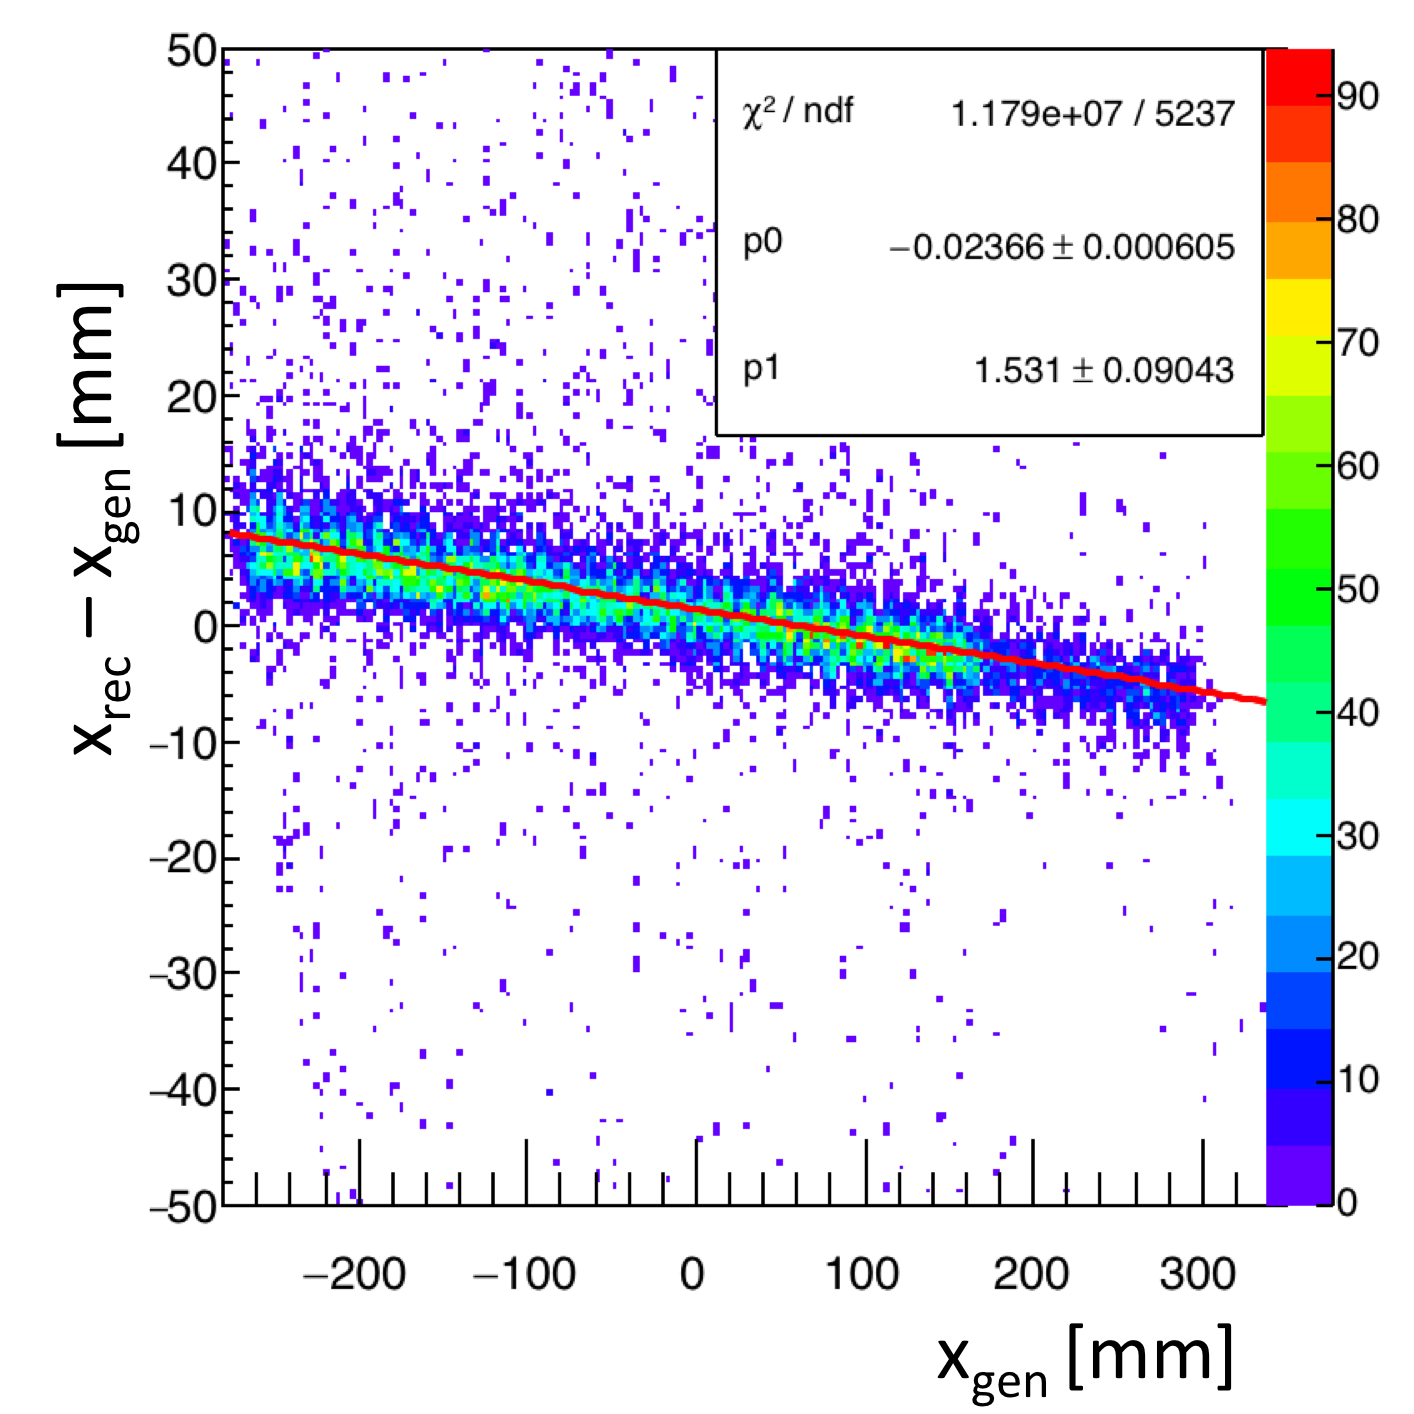
\includegraphics[width=0.7\textwidth]{pics/performance/xposn1gev.png}
  \caption[Horizontal position correction for 1~GeV electrons]{The position correction for 1~GeV electrons plotted versus the Monte Carlo generated position at the ECal. It is both energy and position-dependent in order to account for the different angles of incidence at the ECal.}
  \label{Figure:xposn1gev}
\end{figure}
\indent Additional effects resulting from the differing angles of entry at the ECal require a position correction to the $x$-coordinate of the cluster. These corrections are both charge and momentum-dependent. The position correction for a generated 1~GeV electron is shown in Figure~\ref{Figure:xposn1gev}. The correction at each energy by particle-type is fit with
\begin{equation}
\label{eq:posncorr}
x_{rec} - x_{gen} = A(E_{rec}) x_{gen} + B(E_{rec})
\end{equation}
where the energy-dependence of the fit parameters $A(E_{rec})$ and $B(E_{rec})$ uses the reconstructed cluster energy, uncorrected for shower loss effects. These parameters for the electron horizontal position correction as a function of the reconstructed cluster energy are shown Figure~\ref{Figure:xposcorrPar}.

\begin{figure}[htb]
  \centering
      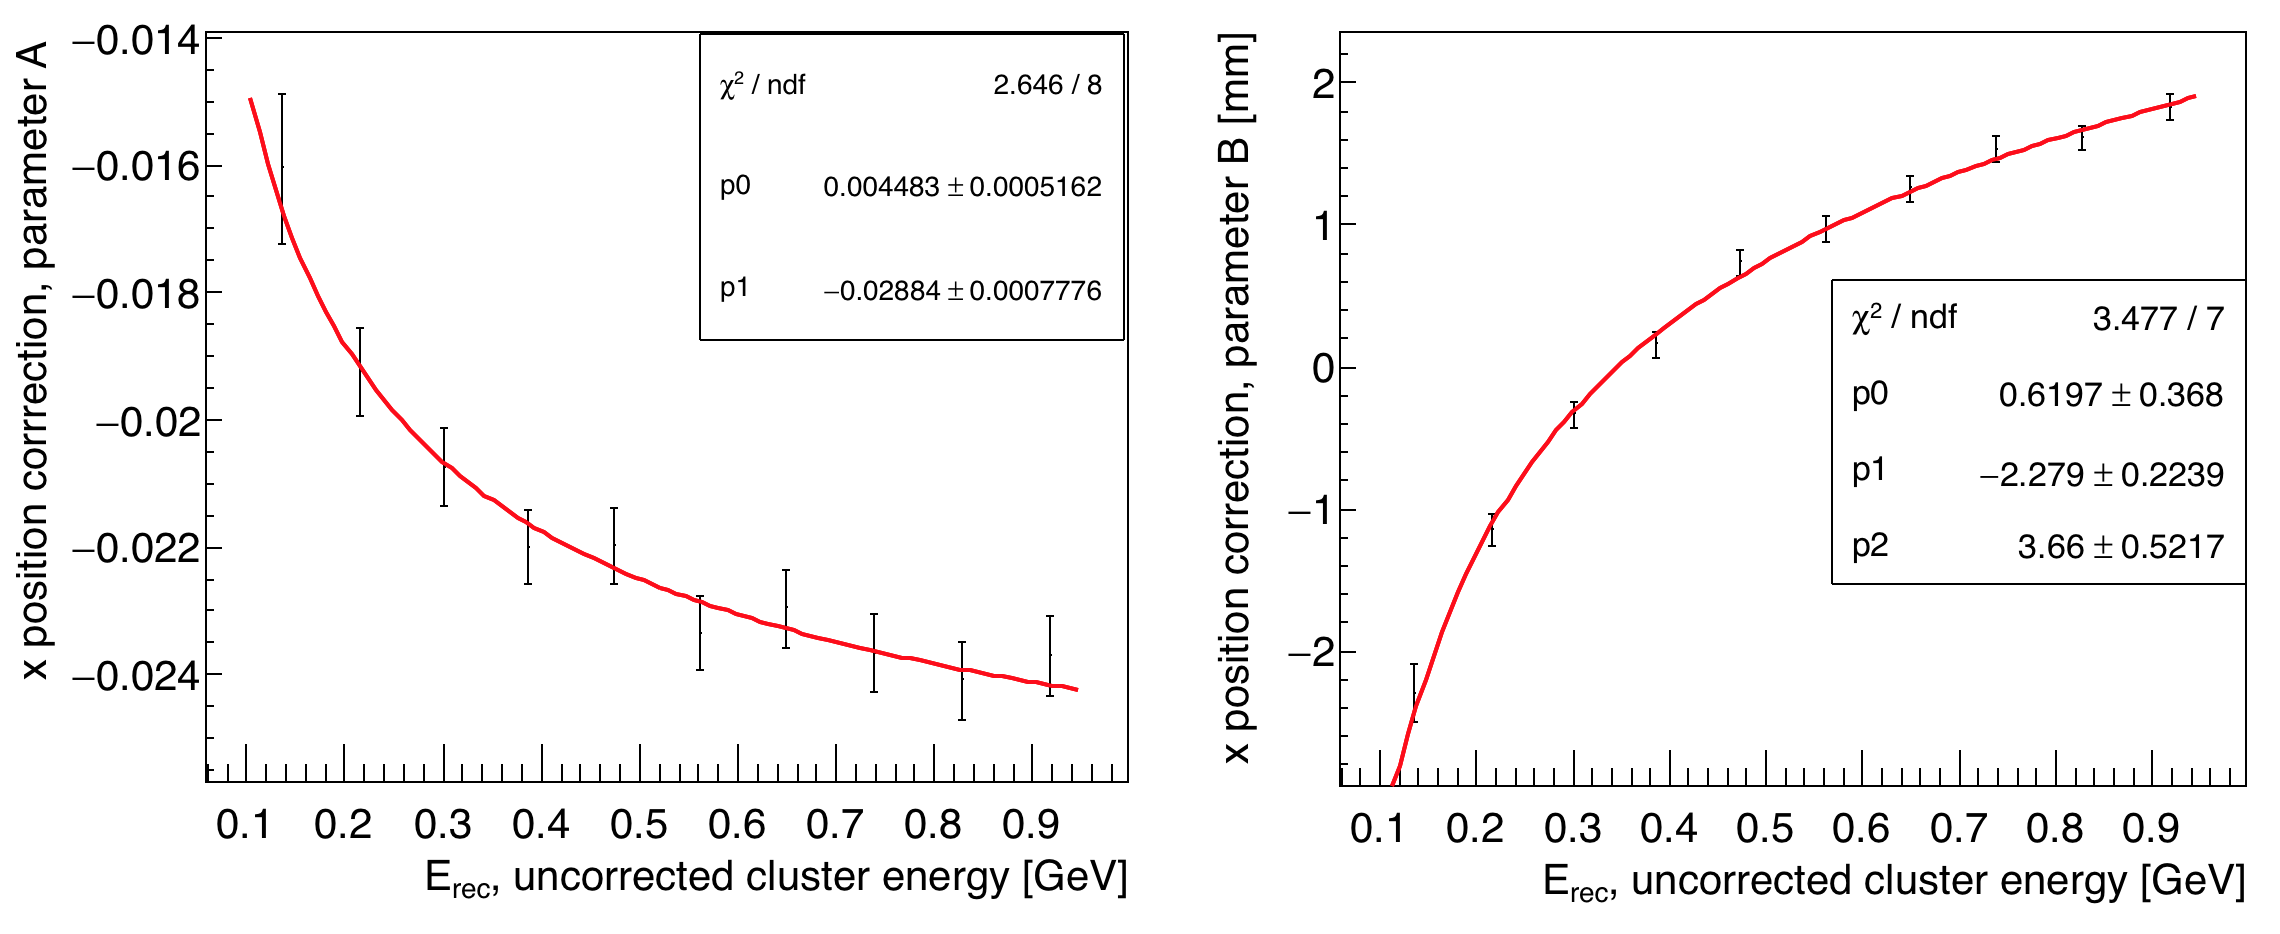
\includegraphics[width=1.0\textwidth]{pics/performance/xposcorrPar.png}
  \caption[Horizontal position correction dependence for electrons]{The horizontal position correction parameters of Equation~\eqref{eq:posncorr} as functions of the reconstructed cluster energy (without any further energy corrections for shower loss).}
  \label{Figure:xposcorrPar}
\end{figure}

The parameters in Figure~\ref{Figure:xposcorrPar} are fit to functions of the form:
\begin{equation}
\label{eq:posnCpar}
\begin{split}
A(E_{rec}) & =  \dfrac{p0}{\sqrt{E_{rec}}}+p1\\
B(E_{rec}) & =  p0\times E_{rec} +\dfrac{p1}{\sqrt{E_{rec}}}+p2
\end{split}
\end{equation}
The correction values for all three particle types are summarized in Table~\ref{tab:horizPosCorr}. Position corrections are not needed for the vertical cluster position.

\begin{table}[htb]
\caption{Horizontal position corrections.}
\label{tab:horizPosCorr}
\centering
\begin{tabular}{|c|c|c|}
\toprule
%\multicolumn{2}{c}{Name} \\
%\cmidrule(r){1-2}
Particle & $A(E_{rec})$ & $B(E_{rec})$ \\
\midrule
electron & $0.004483/\sqrt{E_{rec}}-0.02884$ & $0.6197E_{rec}-2.279/\sqrt{E_{rec}}+3.66$ \\
positron & $0.006887/\sqrt{E_{rec}}-0.03207$ & $-0.8048E_{rec}+0.9366/\sqrt{E_{rec}}+2.628$ \\
photon & $0.005385/\sqrt{E_{rec}}-0.03562$ & $-0.1948E_{rec}-0.7991/\sqrt{E_{rec}}+3.797$ \\
\bottomrule
\end{tabular}
\end{table}


\subsubsection{Position resolution}

After applying the position corrections to each particle-type at the simulated energies, the residual between the measured and simulated position reconstruction is obtained. The fitted residuals for the position of 1~GeV electron clusters are shown in Figure~\ref{Figure:corrPosnsFits}.
\begin{figure}[htb]
  \centering
      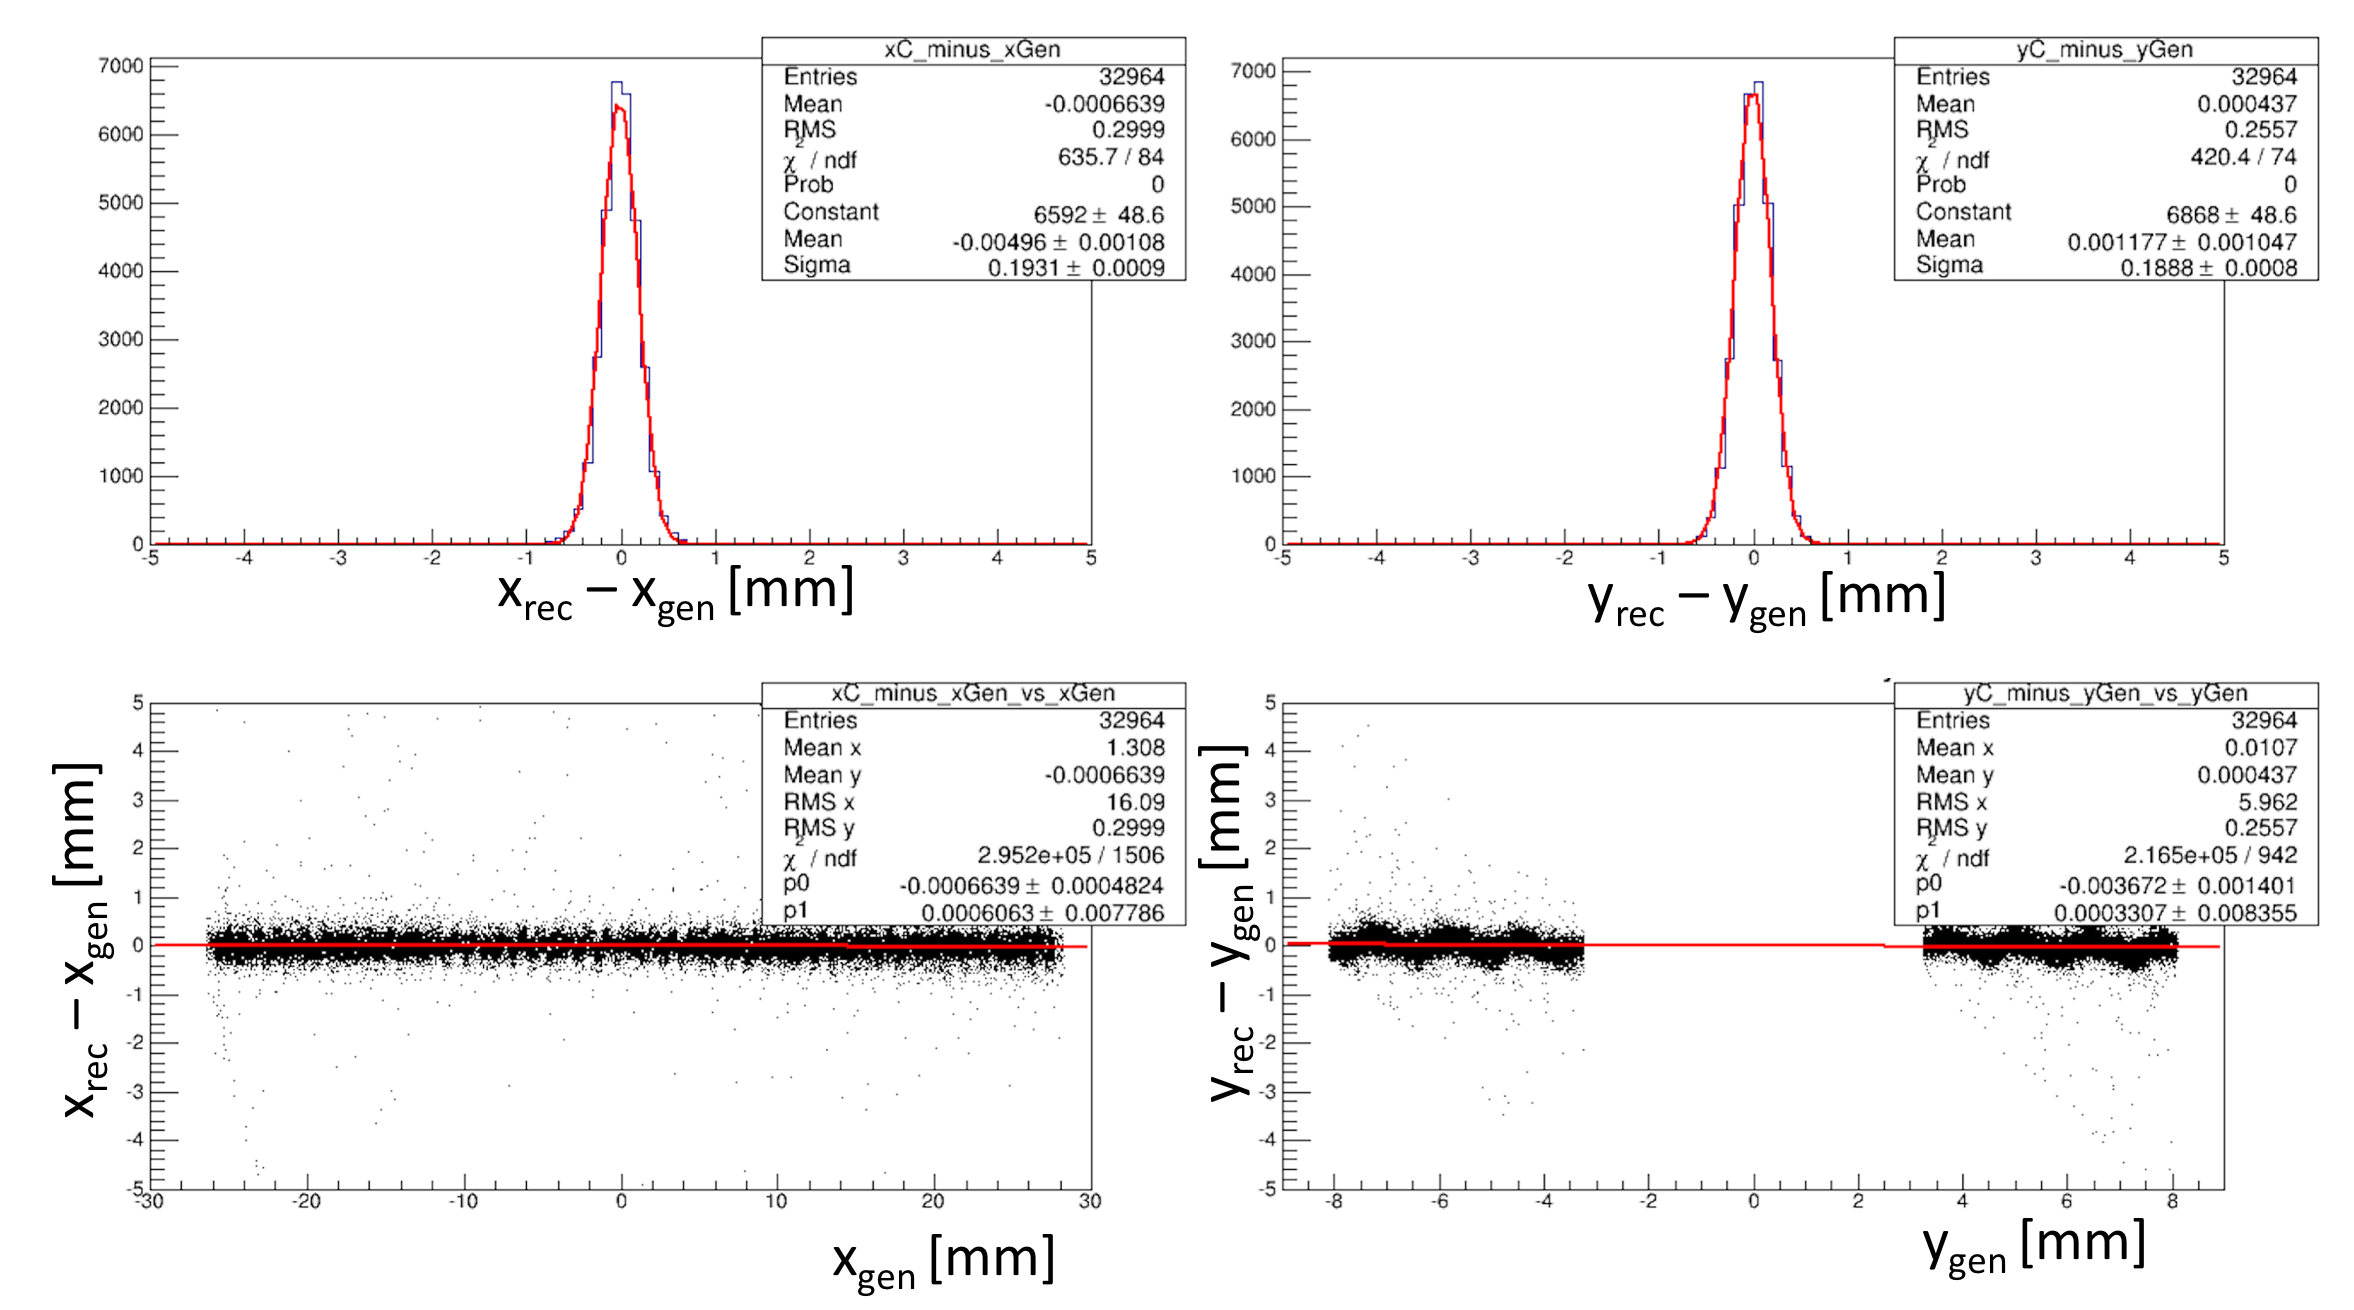
\includegraphics[width=1.0\textwidth]{pics/performance/corrPosnsFits.png}
  \caption[Position resolution for 1~GeV electrons]{The position resolution for 1~GeV electrons, after applying the horizontal position corrections.}
  \label{Figure:corrPosnsFits}
\end{figure}
As shown in Figure~\ref{Figure:corrPosnsFits}, no correction is required when reconstructing the vertical position of the cluster. The energy-dependent resolution of both the horizontal and vertical position of reconstructed clusters can be seen for electrons in Figure~\ref{Figure:emPosnResn}. 
\begin{figure}[htb]
  \centering
      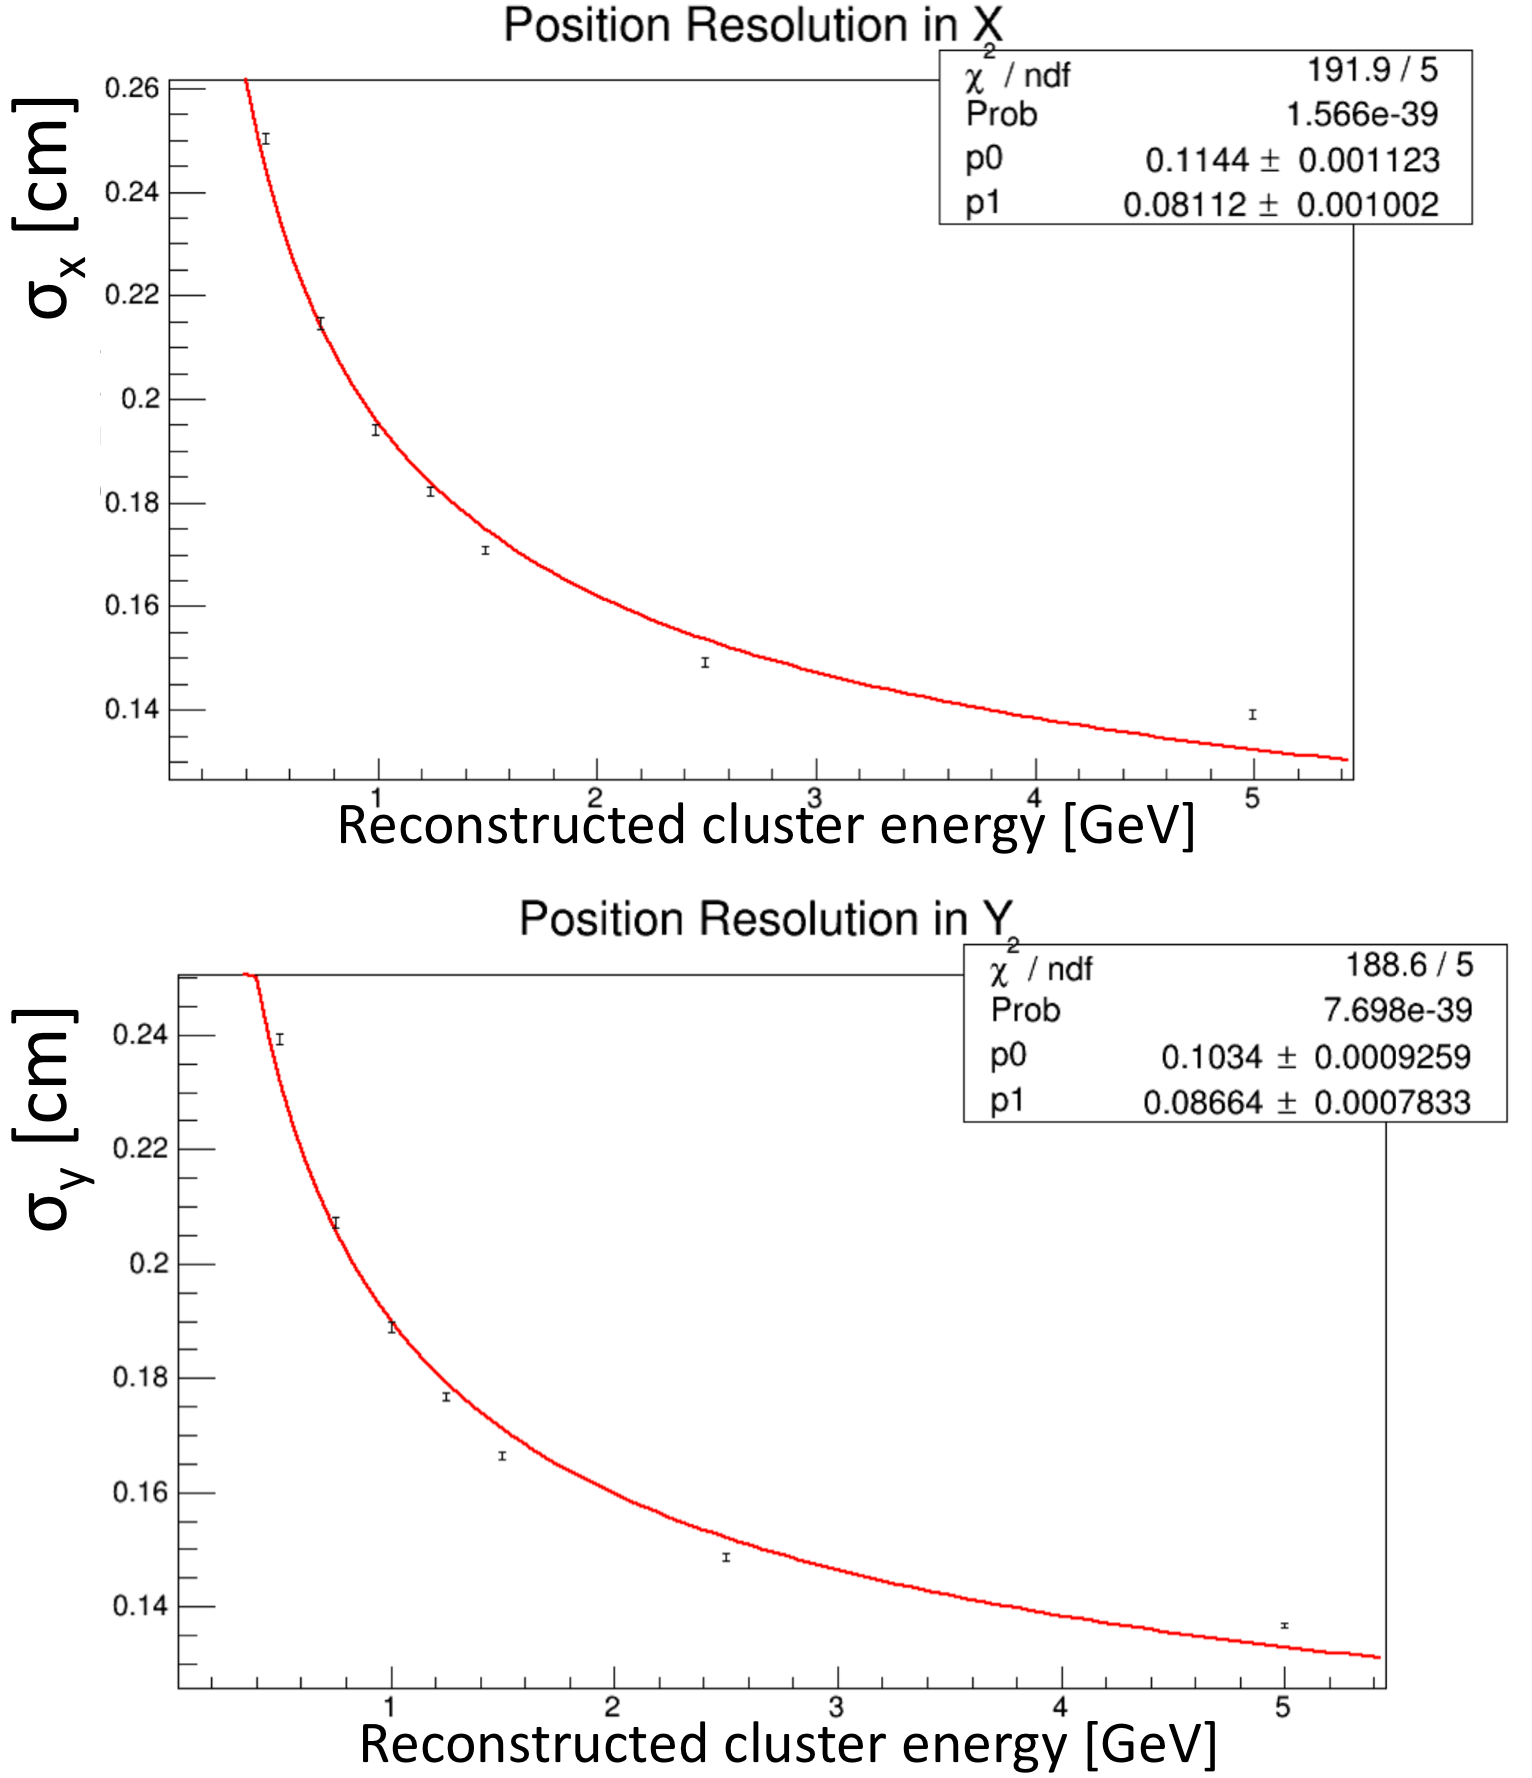
\includegraphics[width=0.7\textwidth]{pics/performance/emPosnResn.png}
  \caption[Energy-dependent position resolution for electrons]{The energy-dependence of the position resolution for electrons as determined from simulation.}
  \label{Figure:emPosnResn}
\end{figure}
The position resolution is parameterized as:
 
\begin{equation}
\label{eq:posnRes}
\begin{split}
\sigma_x \textrm{[cm]}& =  \dfrac{p0_x}{\sqrt{E}}+p1_x\\
\sigma_y \textrm{[cm]}& =  \dfrac{p0_y}{\sqrt{E}}+p1_y
\end{split}
\end{equation}
where the parameters $p0$ and $p1$ are fit to the position resolution as a function of energy. The position resolution is better than 2~mm for 1~GeV electrons. As the ECal face is located at  approximately 1.4~m from the target, the ECal provides valuable position information when matched with a track. The ECal position resolution functions for all particle types is given in Table~\ref{tab:PosnResTable}. The reconstructed cluster energy ($E_{rec}$ in units of GeV) is not corrected for shower-loss effects. 

\begin{table}[htb]
\caption{Position resolution.}
\label{tab:PosnResTable}
\centering
\begin{tabular}{|c|c|c|}
\toprule
%\multicolumn{2}{c}{Name} \\
%\cmidrule(r){1-2}
Particle & $\sigma_x$ [mm] & $\sigma_y$ [mm] \\
\midrule
electron & $0.1144/\sqrt{E_{rec}}+0.08112$ & $0.1034/\sqrt{E_{rec}}+0.08664$ \\
positron & $0.1268/\sqrt{E_{rec}}+0.07711$ & $0.1068/\sqrt{E_{rec}}+0.08423$ \\
photon & $0.1255/\sqrt{E_{rec}}+0.08877$ & $0.1005/\sqrt{E_{rec}}+0.08867$ \\
\bottomrule
\end{tabular}
\end{table}
\subsection{Energy Calibration using cosmic rays}
\begin{figure}[htb]
  \centering
      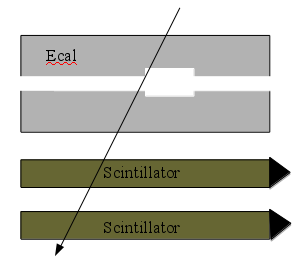
\includegraphics[width=0.7\textwidth]{pics/performance/cosmicschematic.png}
  \caption[Setup for ECal cosmic ray calibration]{Experimental setup for the cosmic ray calibration. The event read out was triggered by the coincidence of the two scintillators.}
  \label{Figure:cosmicScheme}
\end{figure}
The large area APDs enabled the ECal to have the sensitivity to detect signals from cosmic muons traversing the ECal crystals perpendicularly. This signal was used for the initial calibration of the modules. The experimental setup for the cosmic calibrations used two scintillators placed below the ECal to trigger readout of all of the crystals. A schematic for the setup of the cosmic calibration is shown in Figure~\ref{Figure:cosmicScheme}. Each scintillator measures 75~cm long, 22~cm wide and 5~cm thick, covering a slightly larger perpendicular area than the ECal crystals. The two scintillators are less than half a meter apart with the closest scintillator less than half a meter beneath the ECal. \\
\indent The rates and energy deposited in the crystals from cosmic ray muons was studied using Monte Carlo simulation. The energy deposited in each crystal in a layer is proportional to the path length of the track passing through the crystal. From simulation, the average energy deposited in a crystal by a cosmic ray passing vertically though the ECal is shown in Figure~\ref{Figure:cosmicEdep}  (i.e., only tracks passing through one crystal in each row were included).

\begin{figure}[htb]
  \centering
      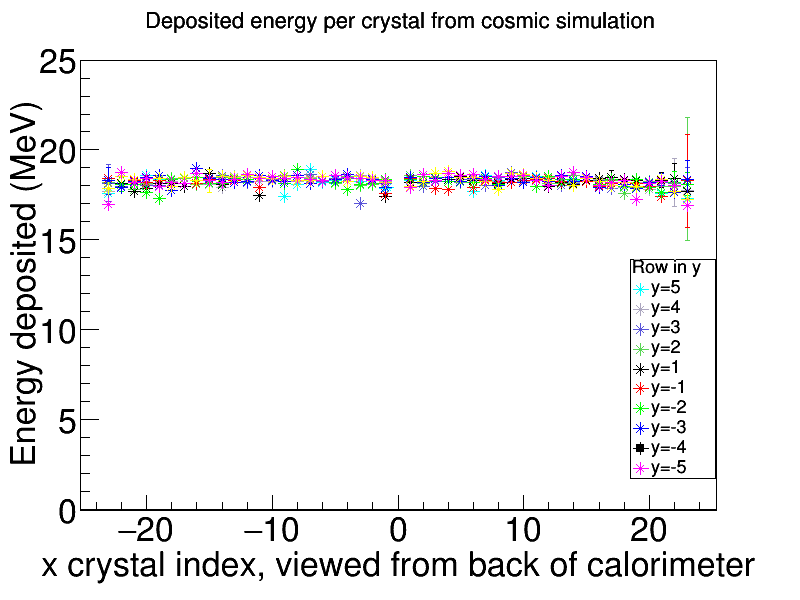
\includegraphics[width=0.8\textwidth]{pics/performance/cosmicEdep.png}
  \caption[Simulation of energy deposited per ECal module from cosmic rays]{The simulated cosmic ray muon energy deposition per crystal of the ECal. The mean energy was 18.3~MeV.}
  \label{Figure:cosmicEdep}
\end{figure}
Additionally, the cosmic ray muon track had to pass through the crystals immediately above and below the struck crystal. For crystals near edges, the geometrical requirement was adjusted to include the two crystals immediately above (or below for cases where the edge is above the crystal) the crystal being read out. The average energy deposited per crystal is approximately 18.3~MeV~\cite{Agashe:2014kda}. In data, the raw FADC waveform for each crystal is read out, and the event is kept for further study after applying strict coincidence cuts between the two scintillators. The trigger rate for data is about 7~Hz. 30$\%$ of events passed the coincidence cut between the scintillators. For a track passing vertically through all ten ECal layers, we can see the signal in each crystal as shown in Figure~\ref{Figure:cosmicSig}.

\begin{figure}[htb]
  \centering
      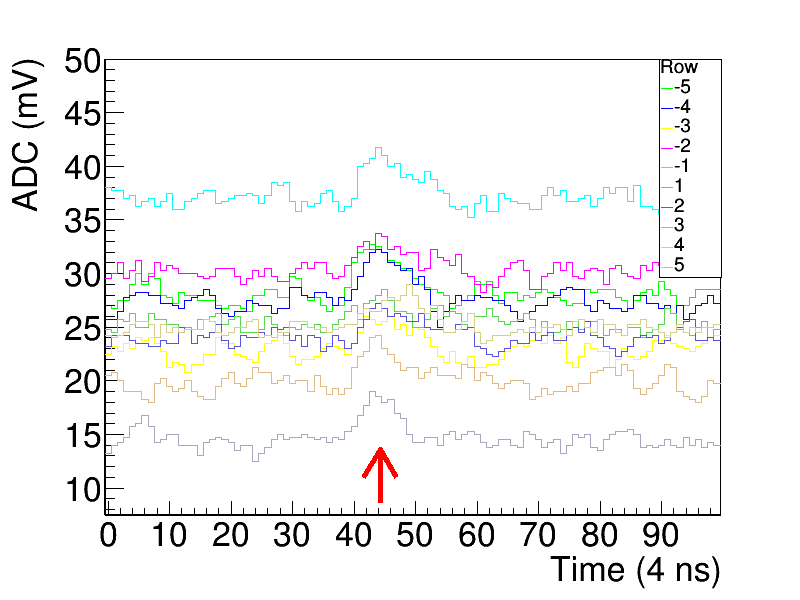
\includegraphics[width=0.7\textwidth]{pics/performance/cosmicSignal.png}
  \caption[Real cosmic ray signal in raw FADC waveform passing vertically through ECal]{The crystal signals plotted versus time for a cosmic ray signal passing vertically through all ten layers of crystals in the ECal. Each crystal's signal is separated vertically in this plot by its pedestal. The arrow indicates the approximate time that the cosmic signal passed through the detector. 1~V corresponds to 4096 FADC channels.}
  \label{Figure:cosmicSig}
\end{figure}

As seen in Figure~\ref{Figure:cosmicSig}, each FADC channel has a different pedestal value. The pedestal for each event was calculated as an average of twenty bins toward the beginning of the time window. By searching for a threshold crossing in the time window where cosmic events occurred, the signal was then fully integrated and the pedestal was subtracted\footnote{The raw waveform thresholds were 2.5~mV in 2015 and increased to 3.5~mV in 2016 to accommodate the larger signals after the removal of the splitters. As shown in Figure~\ref{Figure:readoutChain}, the $1/3$ of the signal from the ECal was split to go to the TDC modules. The splitters and TDCs were removed for the 2016 engineering run so that the full signal could be measured by the FADC.}. Geometric cuts are then applied to the data in offline analysis. Crystals having peaks over a certain threshold must have at least an adjacent crystal located both above and below with a threshold crossing, but the signals in the crystals to the left and right must not cross threshold. These cuts ensure that the track passed as vertically as possible through the ECal (reducing the variation in path length through each crystal). A fit to the energy spectrum in a single crystal is shown in Figure~\ref{Figure:cosmicFit}.\\
\begin{figure}[htb]
  \centering
      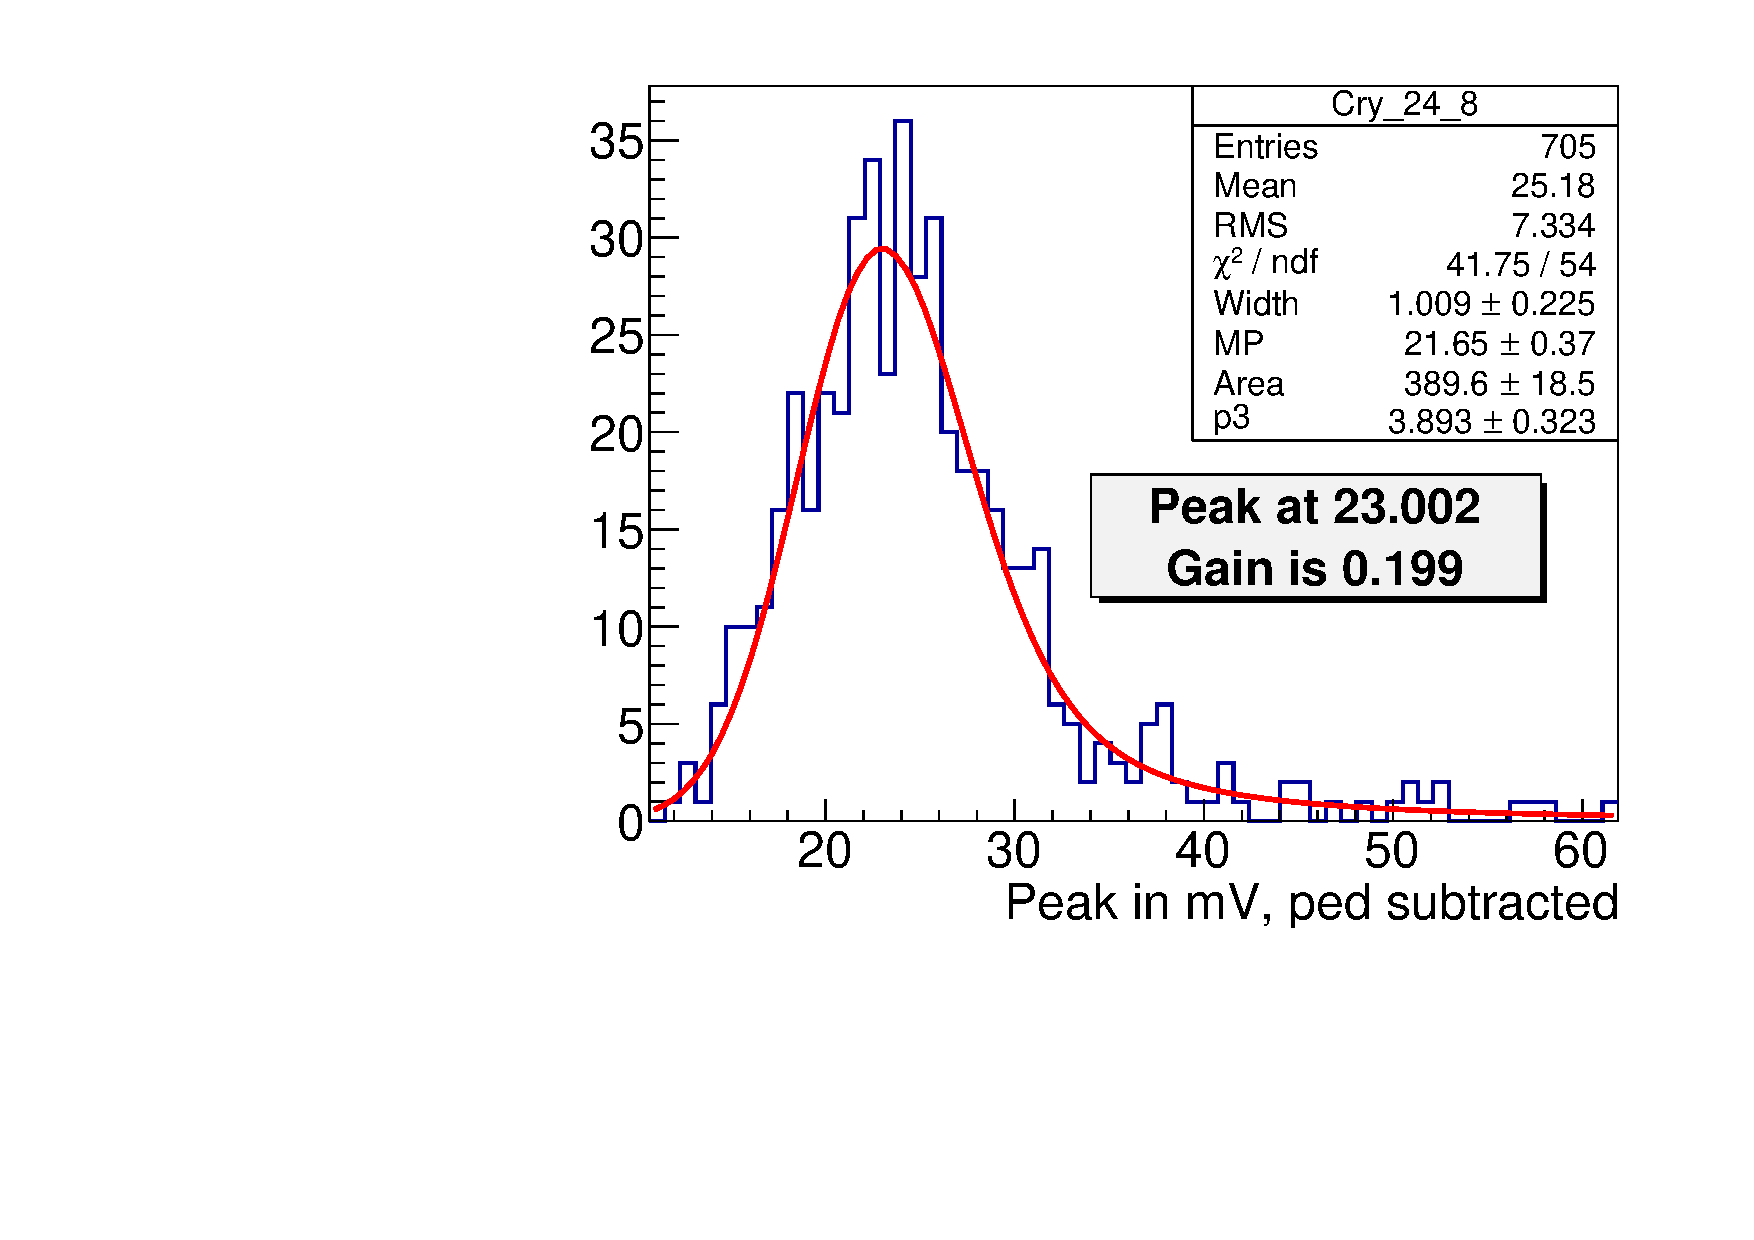
\includegraphics[width=0.8\textwidth]{pics/performance/cosmicFitExample2015.pdf}
  \caption[Integrated cosmic signal in ECal fitted for calibration]{A histogram of the energy (signal pulse integral) deposited by cosmic ray signals in a single crystal. The fit used a Landau-Gaussian convolution function. The peak location was calculated numerically from this fit.}
  \label{Figure:cosmicFit}
\end{figure}
The fit shown in Figure~\ref{Figure:cosmicFit} utilized a Landau-Gaussian convolution as the Landau part corresponds to the crystal's response to a particle's energy deposition, and the Gaussian part accounts for the statistical nature of the electronics shaping and readout. The peak of the fit is calculated numerically, and the initial conversion from pulse-height to energy (MeV) is obtained (called the Gain factor). The gain factor is calculated using the measured peak position in units of FADC pulse-integral and the known energy deposited from the simulation in units of MeV:
%1~V corresponds to 4096~FADC channels. The 4096~FADC counts can be set to 1~V or 2~V, but for 2015 and 2016 running, the setting was 1~V. 
\begin{equation}
	\label{eq:gain}
	\textrm{Gain} = \dfrac{\textrm{[MeV]}}{\textrm{[FADC pulse-integral]}} 
\end{equation}
The full ECal was calibrated with about 60~hours of cosmic ray data. The resultant gains for all channels in the 2015 engineering run are shown in Figures~\ref{Figure:cosmicG} and~\ref{Figure:cosmicGhisto}.

\begin{figure}[htb]
  \centering
      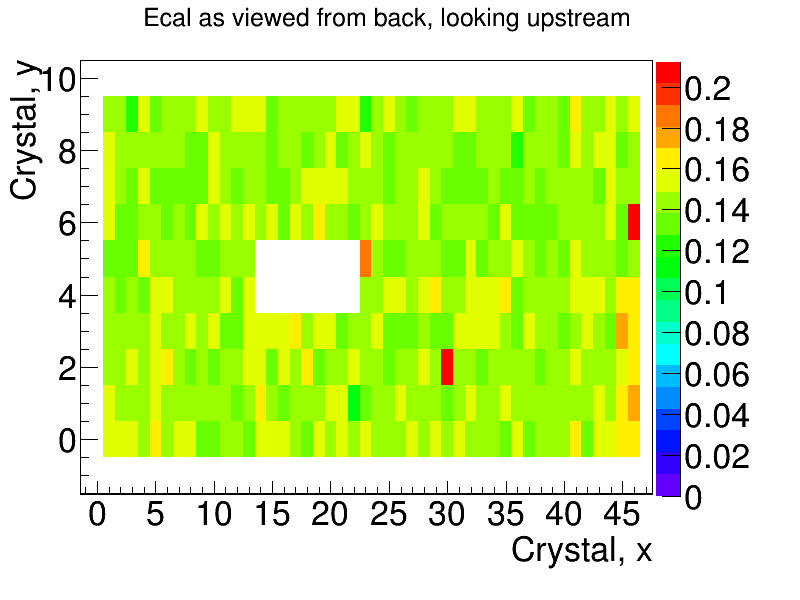
\includegraphics[width=0.7\textwidth]{pics/performance/cosmicGains2015.png}
  \caption[Resulting 2015 gain calibration in the ECal using cosmic ray muons shown by ECal module position]{Resulting gain calibration for each crystal using cosmics for the 2015 engineering run where the $z-$axis color is shown in units of [MeV/FADC pulse-integral].}
  \label{Figure:cosmicG}
\end{figure}


\begin{figure}[htb]
  \centering
      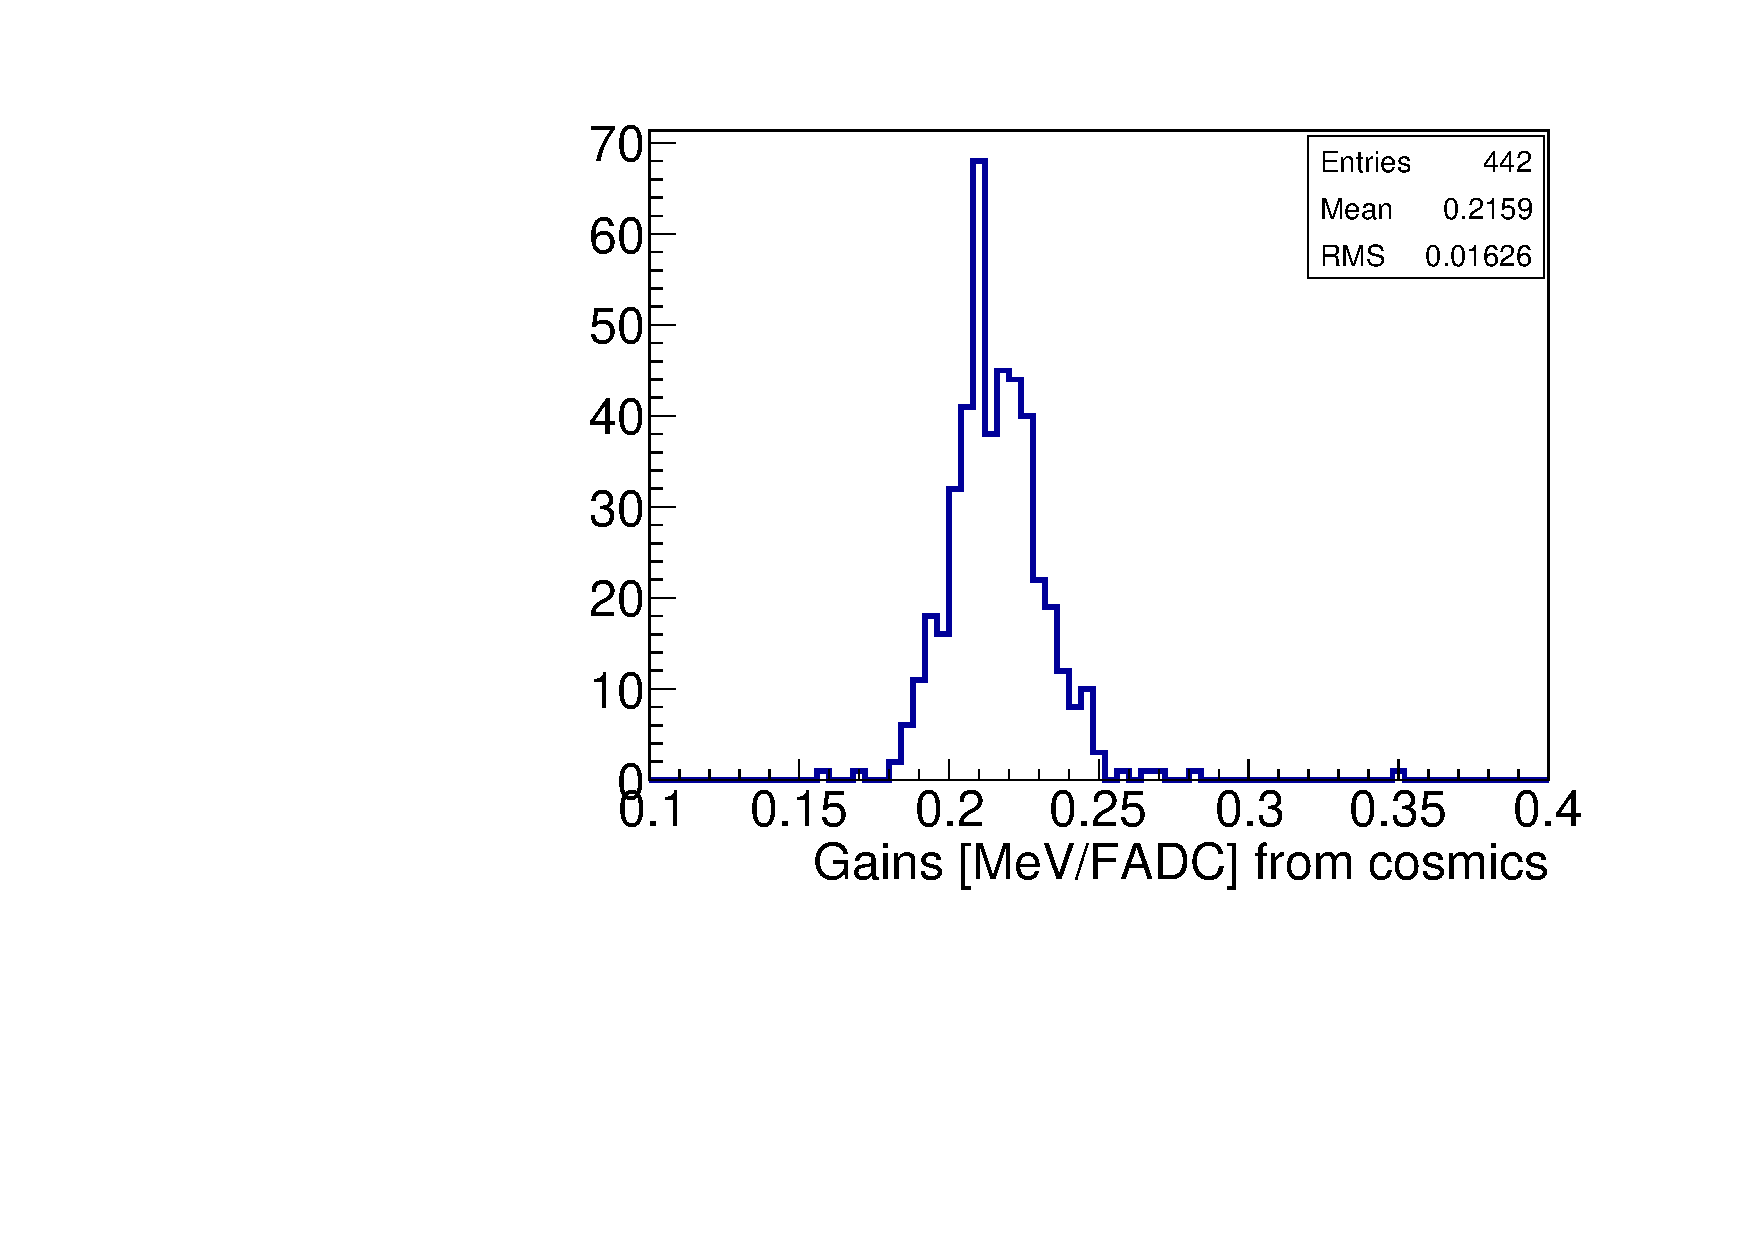
\includegraphics[width=0.7\textwidth]{pics/performance/cosmicGainsMay15.pdf}
  \caption[Distribution of the resulting 2015 gains in the ECal using cosmic ray muons]{Resulting gain calibration for all crystals using cosmics for the 2015 engineering run.}
  \label{Figure:cosmicGhisto}
\end{figure}

With the splitters installed in the ECal readout chain (shown in Figure~\ref{Figure:readoutChain}), the average gain value was around 0.2~MeV/FADC pulse-integral for the 2015 engineering run. After the removal of the splitters in January 2016, prior to the spring run, the average gains were found to be around 0.13~MeV/FADC pulse-integral.

\subsection{Ecal signal pulse fitting} \label{pulsefitting}
All data was taken using the FADC250 modules which sample at 250~MHz, or every 4~ns. While the firmware has various modes for recording data, data size was not an issue and Mode 1 was used during both engineering runs. Mode 1 preserves the full measured waveform for a module hit to allow for improved methods for extracting the energy and time information in offline analysis. The trigger decision to read out a module is based off a leading edge threshold which was set to 12~FADC pulse-height units in the 2015 engineering run. \\
\indent The full response for each module was carefully studied in order to understand the time response and shaping effects of the preamplifier on the ECal modules \cite{charles_2014}. The raw waveform response was best described by the sum of the pedestal $P$ and a $3$--pole function for the pulse with width $\tau$ occurring at time $t_0$:

\begin{equation}
	\label{eq:thrpole}
	E(t) = P + \dfrac{A}{2\tau^3}(t-t_0)^2e^{-(t-t_0)/\tau} 
\end{equation}
where the pulse integral value is the parameter $A$. When $t<t_0$, the pulse amplitude is zero. The best resolutions were found by fixing the width parameter for each module as the average measured over several pulses. An example fit is shown in Figure~\ref{Figure:mode1fit}.

\begin{figure}[htb]
  \centering
      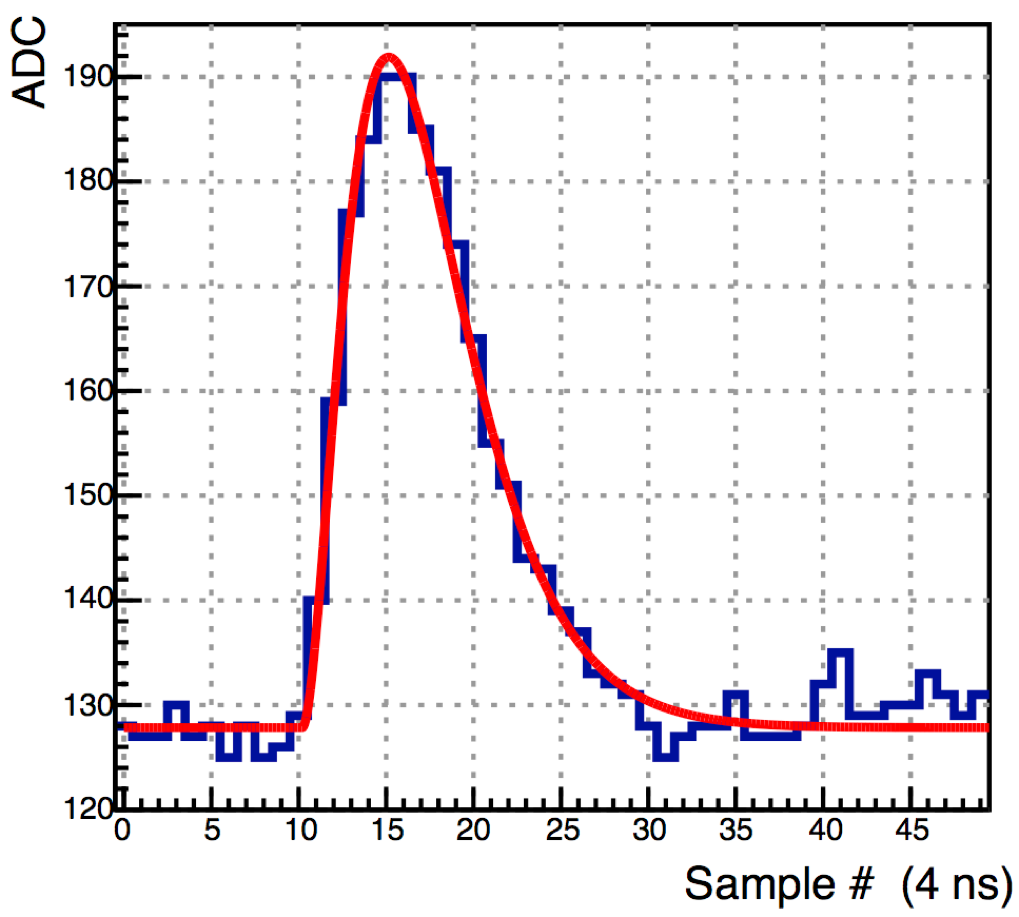
\includegraphics[width=0.5\textwidth]{pics/performance/mode1fit.png}
  \caption[Pulse-fitting to Mode 1 ECal data]{Example fit to a real ECal module pulse.}
  \label{Figure:mode1fit}
\end{figure}

The pedestal is calculated event-by-event and initialized by a running average over the previous fits for the pulse. The fit range was set to 20~ns before and 60~ns after the threshold crossing in order to eliminate contamination from pile-up signals in the same event~\cite{baltzell_ecal_2015}. The offline pulse-fitting of the raw waveform demonstrated the best time resolution and energy resolution when compared to the other hardware integral methods that could have been implemented~\cite{baltzell_ecal_2015}.

\subsection{Calibration using elastically-scattered electrons}
The calibration using cosmic ray muons was sufficient for initial data-taking with the electron beam, but the overall energy calibration of the ECal is optimal at higher energies. The ECal detects elastically scattered electrons that peak, after correction for shower leakage effects, at the beam energy. As the target is off centerline beam right, there are geometric effects that prevent elastically-scattered beam energy electrons from illuminating the entire ECal~\cite{szumila-vance_hps_2016}. From simulation, the rightmost column of crystals, and the five leftmost columns of crystals cannot be calibrated using elastically-scattered electrons. \\
\indent To calibrate the ECal using elastically-scattered electrons, we selected events where the seed hit crystal carried at least 60$\%$ of the overall cluster energy. The seed hit was also required to have more than 450~MeV in the 2015 data (1.1~GeV for the 2016 data), to have triggered a Singles 1 event readout from the DAQ, and to have occurred in the optimal trigger timing window. The cluster energy was associated with the seed hit module for the calibration. The calibration uses an iterative procedure, by which the reconstructed cluster energy is matched to the expected simulated energy (prior to energy corrections). For each crystal's cluster energy, an iteration coefficient is found that reflects the ratio of the cluster energy measured in Monte Carlo to the cluster energy found for that iteration:\\
\begin{equation}
	\label{eq:feeiter}
	C_i = \dfrac{MC_{peak}}{data_{peak}}
\end{equation}
After each iteration, this ratio $C_i$ is applied to the to the original gain coefficient as well as any coefficient found from a previous iteration. The data is re-processed applying these changes to the gains and clustering is re-run. This procedure continues until the correction coefficients found in a particular iteration are all less than 1$\%$. Crystals on the edge of the acceptance with poorly resolved peaks were given an iteration coefficient of 1. After completion of the calibration (approximately 2-3 iterations)~\cite{szumila-vance_hps_2016}, the shower loss correction functions were applied to the reconstructed cluster energies. The measured ECal energy for elastically-scattered electron clusters in the fiducial region of the ECal is shown in Figure~\ref{Figure:FeeFidPeak}.
\begin{figure}[htb]
  \centering
      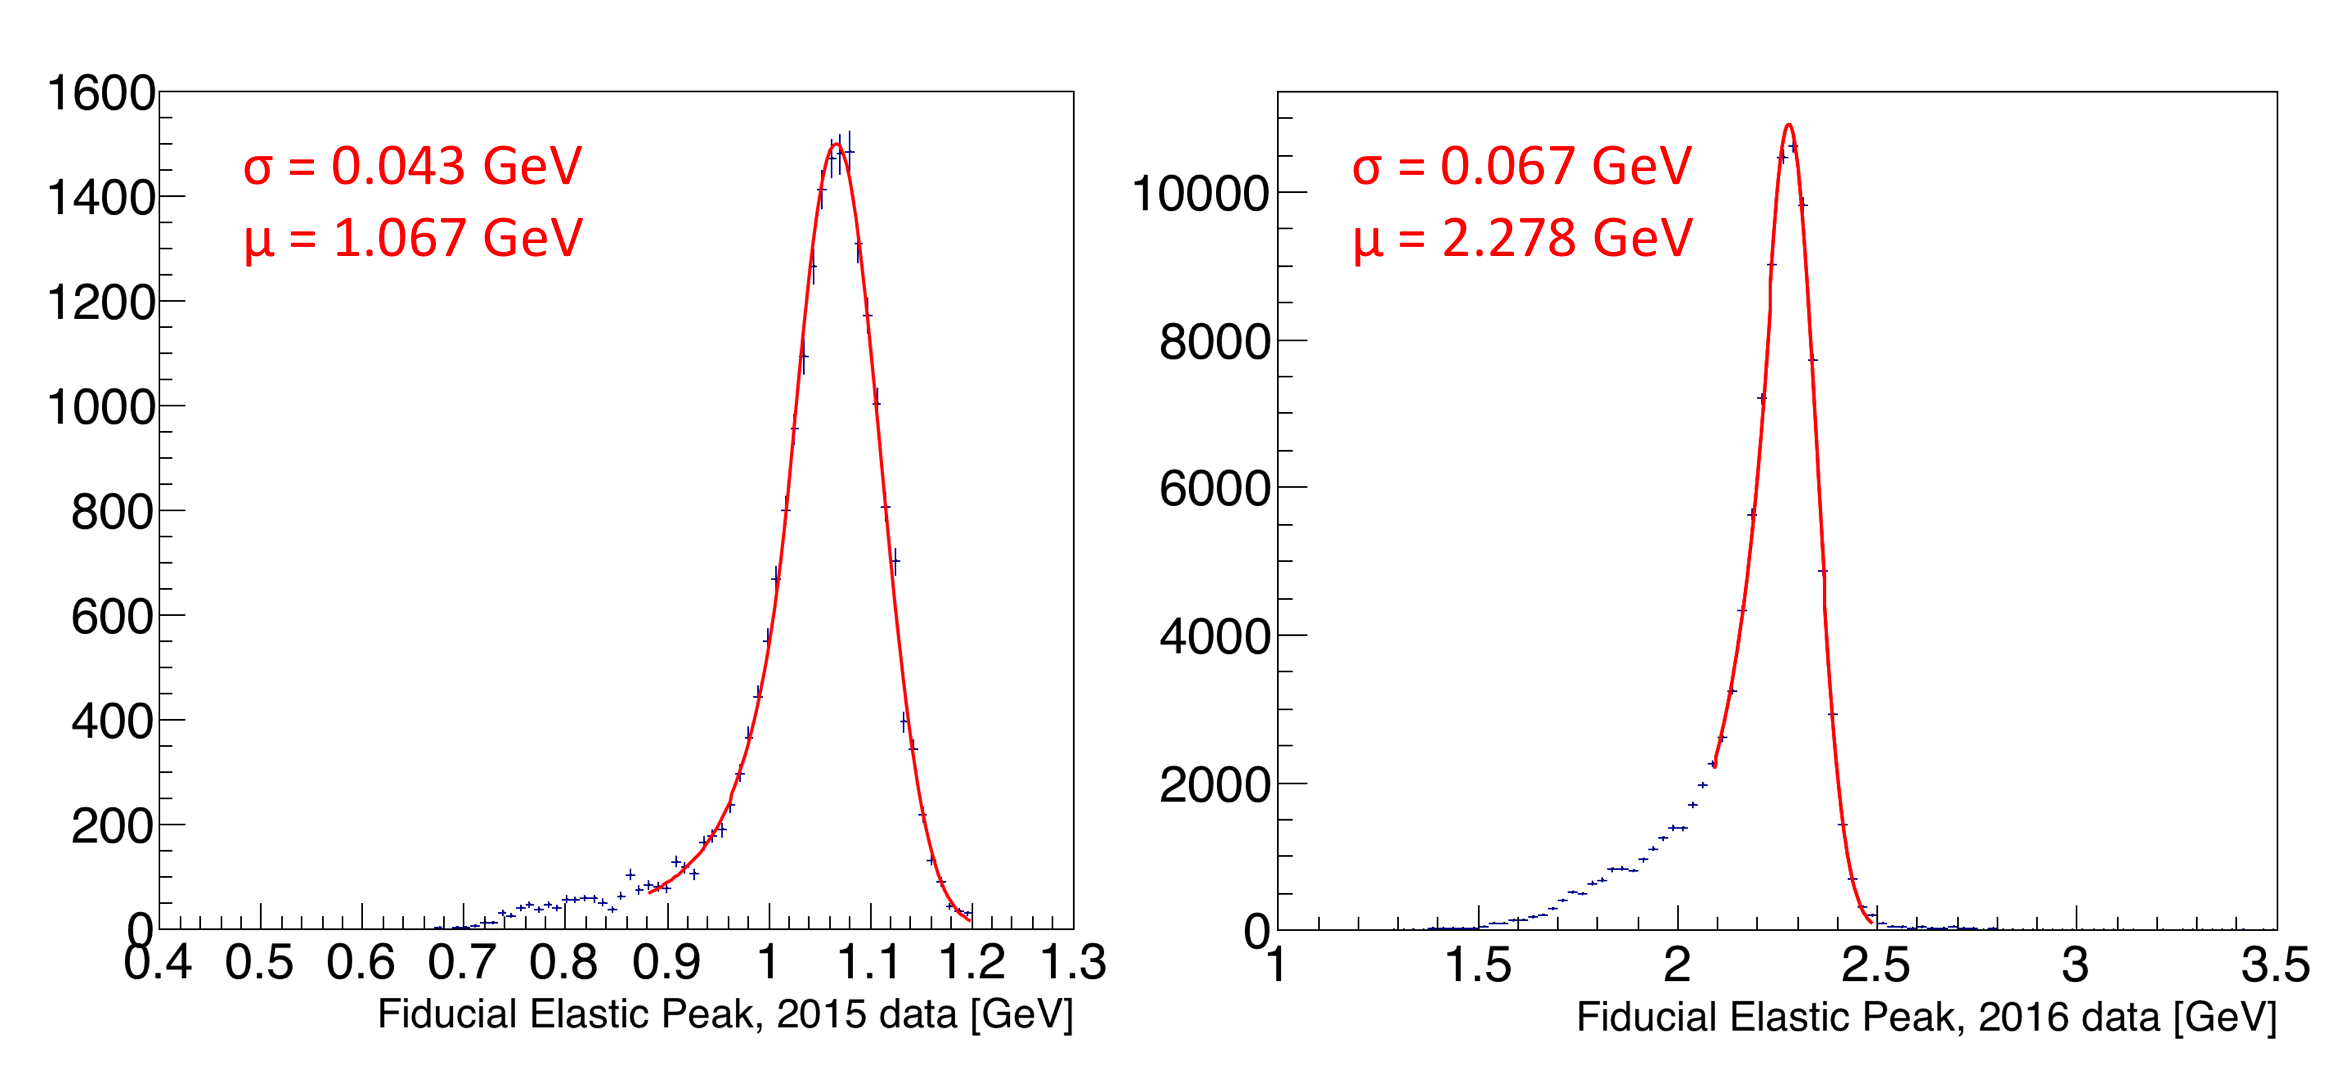
\includegraphics[width=0.9\textwidth]{pics/performance/feePeakFid.png}
  \caption[Reconstructed elastic peak in the ECal for the engineering runs]{The energy deposited in the fiducial region of the ECal for elastically-scattered electrons for the 2015 and 2016 runs is shown on the left and right, respectively. The peaks are fit with a Crystal Ball function and the peak position and widths are indicated. }
  \label{Figure:FeeFidPeak}
\end{figure}
The energy resolution improves with the beam energy. The cluster energy spectrum is fit with a Crystal Ball function which contains a Gaussian component and a power law low energy tail. The ECal has an energy resolution of approximately 4$\%$ in the fiducial region at 1~GeV and 2.9$\%$ at 2.3~GeV. \\
\indent The final gains obtained after calibration with elastically-scattered electrons were compared to the gains obtained with cosmics alone in order to check for systematic offsets. No systematic offsets were found. The comparison between the low and high energy calibrations tells us that cosmic calibration was roughly accurate, but it is limited in telling us anything about how linear the gain response is of the ECal between these two points in energy~\cite{szumila-vance_hps_2016}. Because not all of the crystals are calibrated using elastically-scattered electrons due to acceptance, the gains from cosmics were compared to the gains obtained from elastically-scattered electrons to check that there is no systematic offset. Any systematic difference would need to be applied to the crystals calibrated only with cosmics and the effects on the triggered data would need to be quantified. No systematic offset was observed. 
%\begin{figure}[H]
 % \centering
    %  \includegraphics[width=0.9\textwidth]{pics/performance/cosmicComp.png}
 % \caption[Gain comparison between cosmic and elastic calibration]{A comparison between the gains from he cosmic and elastic calibration is shown. Any overall systematic shift would need to be applied to crystals outside of the elastic calibration acceptance. }
%  \label{Figure:cosmicComp}
%\end{figure}

\subsection{Wide angle bremsstrahlung for studies of edge effects}
The primary physics trigger looks for events with two clusters. However, it also recorded a high yield of WAB events composed of an electron and a photon. The spectrum of cluster energies in the 2015 engineering run data set shows an excess of WAB events occurring where the energy sum of the two particles is approximately equal to the beam energy. \\
\indent Initial studies showed that the energy sum of two particles in WAB events having mid-range energies was lower than the reconstructed elastic energy, indicating that the shower loss corrections in the mid-range beam energy required further investigation. WAB events were used to refine the shower loss corrections for mid-range energy particles. WAB events are identified by having one track-matched cluster and one cluster with no matching track. The reconstructed energy sum of of the two particles must equal the beam energy~\cite{szumila-vance_hps_2016}:
\begin{equation}
	\label{eq:wabBeam}
	E_i = \dfrac{E_{e^-}}{f_{e^-}(E_{e^-})}+\dfrac{E_{\gamma}}{f_{\gamma}(E_{\gamma})}
\end{equation}
where $f$ refers to the shower loss correction described by Equation~\eqref{eq:eclsf}. The underlying assumption is that the relationship between the electron and photon shower loss corrections found in Monte Carlo are preserved:
\begin{equation}
	\label{eq:wabRatio}
	 \dfrac{f_{e^-, data}(E_{e^-})}{f_{\gamma, data}(E_{\gamma})}= \dfrac{f_{e^-, MC}(E_{e^-})}{f_{\gamma, MC}(E_{\gamma})}
\end{equation}
In maintaining the relationships shown in Equations~\eqref{eq:wabBeam} and \eqref{eq:wabRatio}, a chi-squared minimization yields the optimal adjustments to the shower loss correction functions for mid-range energy particles:
\begin{equation}
	\label{eq:wabBeamChi}
	\chi^2 =\sum_{i} \dfrac{(E_{beam}-E_{sum})^2}{\sigma_{e^-}^2(E_{e^-})+\sigma_{\gamma}^2(E_{\gamma})}	
\end{equation}
For each event, the energy sum of the two corrected clusters, $E_{sum}$, is calculated as described by Equation~\eqref{eq:wabBeamChi}. The end result is a small correction to the shower loss correction functions that ranges across the cluster energies and never exceeds 2$\%$~\cite{szumila-vance_hps_2016}. After incorporating these updated corrections to the shower loss correction functions, the energy resolution can be extracted for all energies and positions in the ECal.  

\subsection{Energy resolution in data}\label{EcalResData}
The elastically-scattered electrons provided the cleanest point in extracting the energy resolution of the ECal at the beam energy. Using WAB particles, electrons and photons, the energy resolution of the ECal was characterized for energies less than the beam energy for different positions relative to the edges.\\
\indent To study the energy resolution in the fiducial region of the ECal, all electrons were matched to tracks, and the track position extrapolation to the face of the ECal was used to determine the electron's vertical distance relative to the beam gap edge. For WAB electrons, the photon cluster was required to be at least 10~mm from the ECal edges to avoid edge effects. By selecting WAB events where the energy difference between the two particles is less than 100~MeV, the resolution of the energy sum peak was fitted to extract the resolution. The resolution was extracted:
\begin{equation}
	\label{eq:eResExtract}
	\sigma_{E_{\gamma}+E_{e^-}}^2 = \sigma_{e^-}^2(E_{e^-})+\sigma_{\gamma}^2(E_{\gamma})
\end{equation}
When both particles are in the fiducial region and are roughly equal in energy, then the energy resolution of the sum could be divided by $\sqrt{2}$ assuming that the energy resolution of both particles is the same. This same procedure was used to study the resolution when the particle energies were more asymmetric in energy in order to obtain the single particle energy resolution at various energies. \\
\indent The experimentally-obtained fiducial energy resolution agrees well with Monte Carlo but is about 15$\%$ larger (see Figure~\ref{Figure:eResData}).
\begin{figure}[htb]
  \centering
      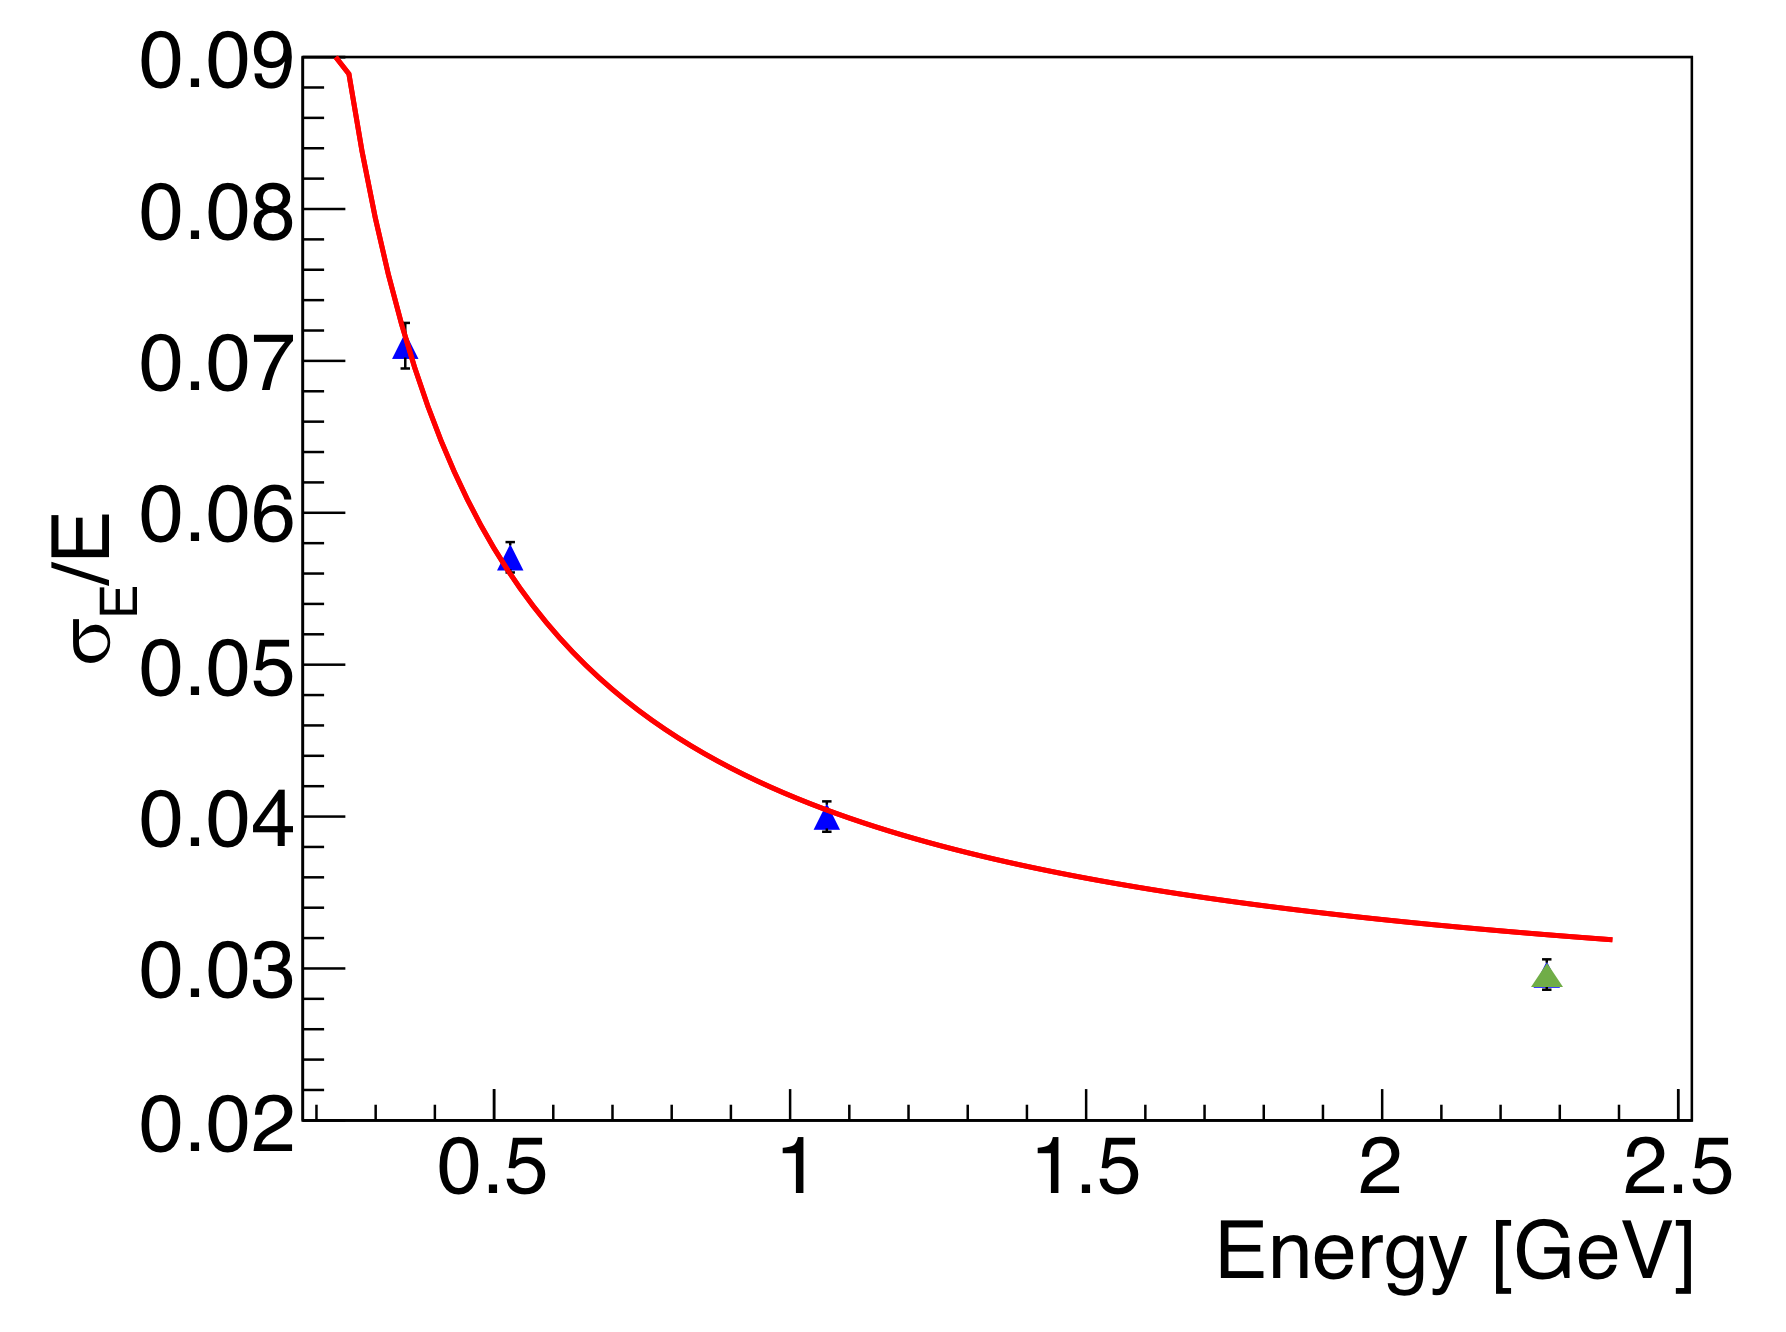
\includegraphics[width=0.6\textwidth]{pics/performance/eResData.png}
  \caption[Energy resolution of the ECal found in data]{The blue points are derived from the 2015 engineering run for the energy resolution of a single particle. The green point at approximately 2.3~GeV was determined from the elastic calibration of the 2016 engineering run data. The energy resolution was fit to the 2015 engineering run data only and extrapolated to higher energies.}
  \label{Figure:eResData}
\end{figure}
The fit to the energy resolution (energy in units of GeV) using the blue points from the 2015 engineering run data in Figure~\ref{Figure:eResData} is:\\
\begin{equation}
	\label{eq:eResData}
	\dfrac{\sigma_E}{E}(\%) = \dfrac{1.62}{E}\oplus\dfrac{2.87}{\sqrt{E}}\oplus2.5
\end{equation}
The first term is attributed to the noise from the pre-amplifiers and is roughly consistent to that found in Monte Carlo. The second term is related to the statistical fluctuations of the shower containment and the APD gain. This term is larger than the term found in Monte Carlo but is still consistent. The third term contains both the energy leakage out the back of the ECal as well as the crystal-to-crystal inter-calibration error. This term is significantly higher than anticipated from Monte Carlo, but is comparable to that found for the IC. It's possible that this term is affected by the inability to calibrate several crystals along the outer edges of the calorimeter with elastic electrons. \\
\indent The energy resolution from the 2.3~GeV engineering run (shown in green on Figure~\ref{Figure:eResData}) is slightly better than that predicted by the fit from the 1.056~GeV engineering run. It is likely that the energy resolution of the ECal improved because the signal going into the FADC modules was no longer split. \\
\indent The WAB events are a useful tool for studying the energy resolution in the ECal as a function of position relative to the edge. By selecting a photon cluster in the fiducial region of the ECal, the energy resolution of the electron (position given by the track projection at the ECal) could be measured at various energies. The second parameter of the energy resolution function described by Equation~\eqref{eq:eResData} (of the form $b/\sqrt{E}$) is strongly correlated with the vertical position relative to the beam gap edge. By fixing the other two terms to the values in the fiducial region, the value of the $b$ parameter was studied as a function of position~\cite{szumila-vance_hps_2016}. The final characterization of this value relative to the beam gap edge is shown in Figure~\ref{Figure:stochasticEdge}~\cite{balossino_hps_2016}.

\begin{figure}[htb]
  \centering
      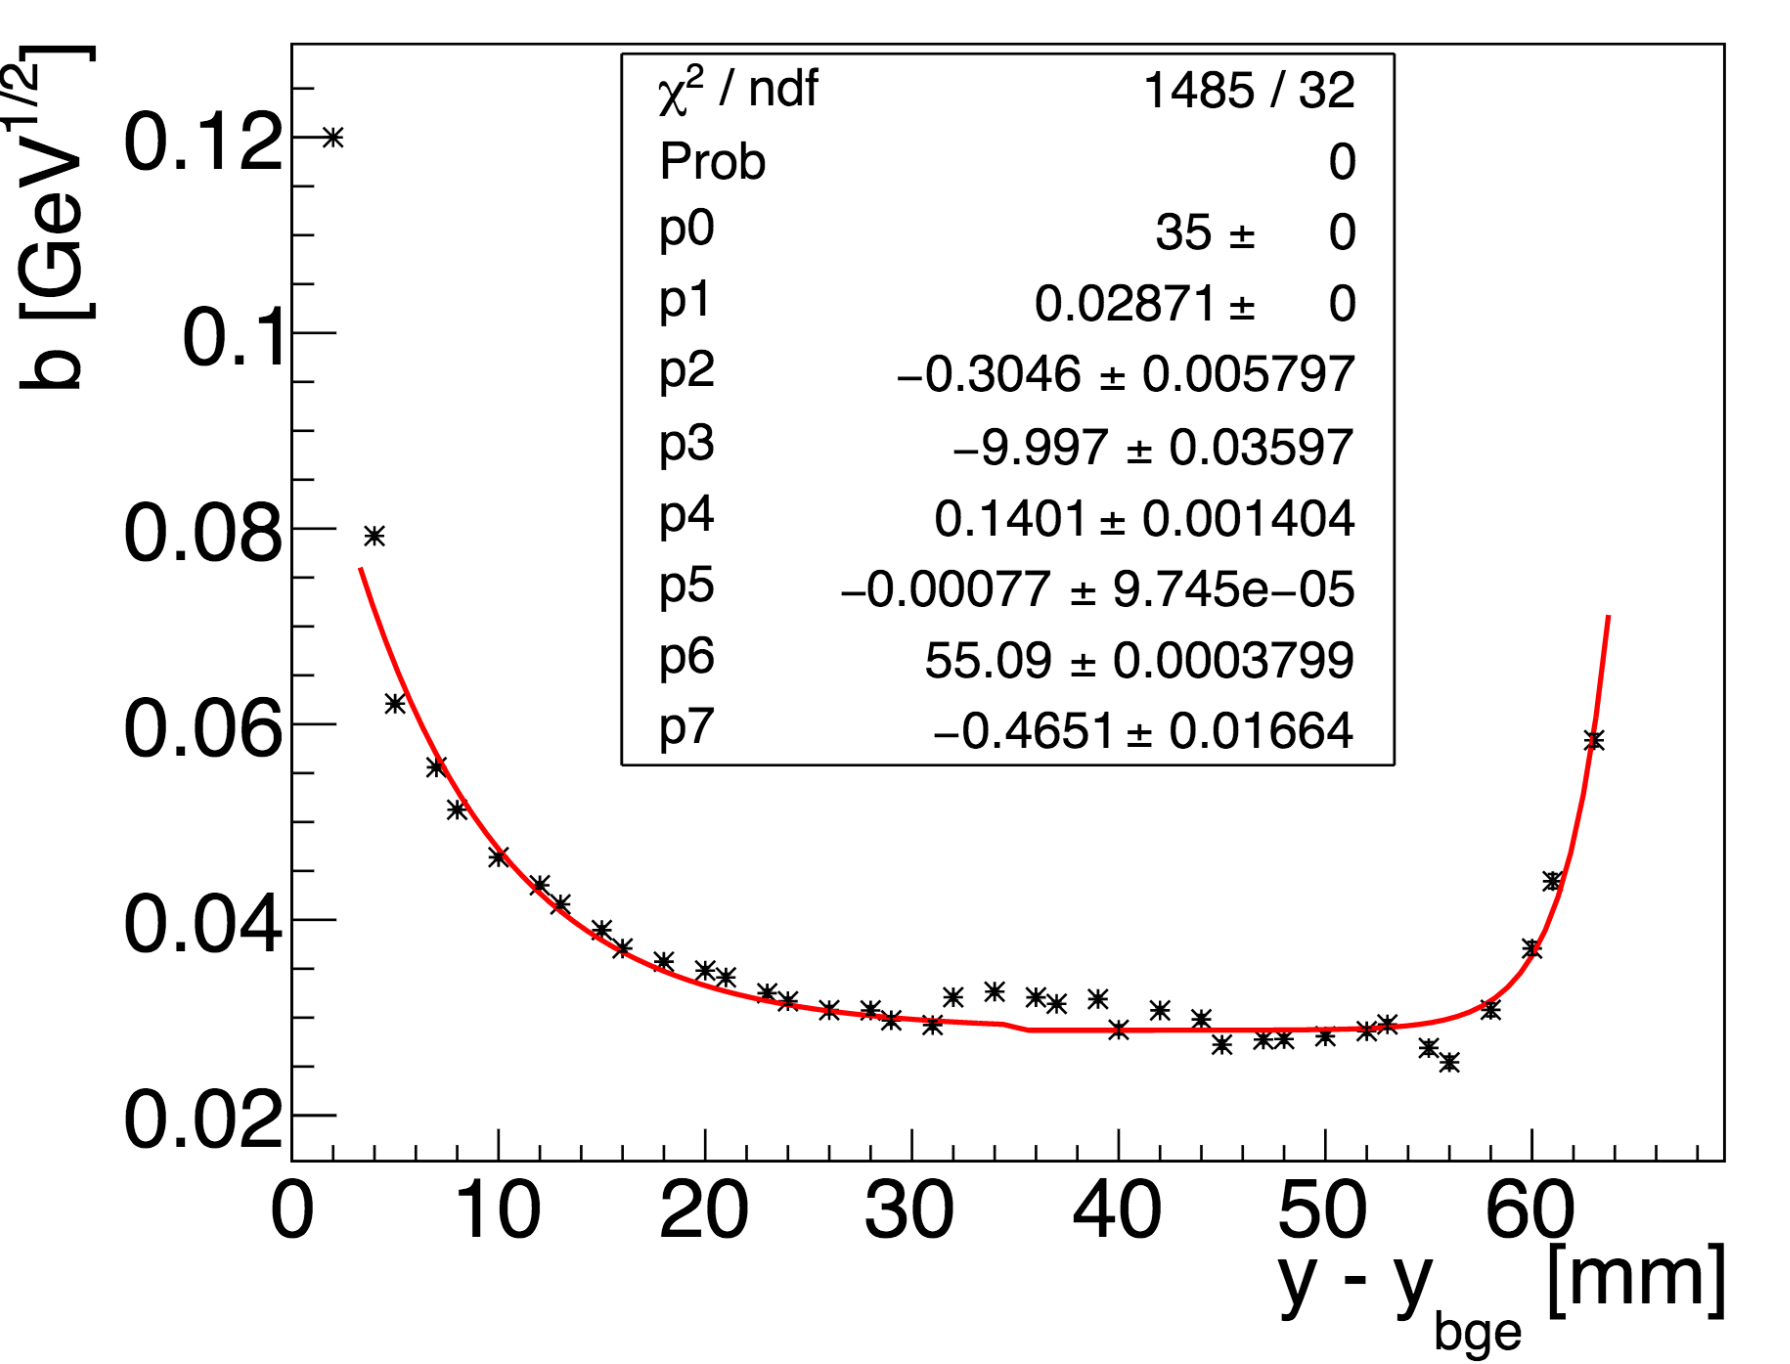
\includegraphics[width=0.5\textwidth]{pics/performance/eResEdgeEffect.png}
  \caption[Characterization of the energy resolution edge effects ]{The stochastic parameter $b$ (corresponding to the $1/\sqrt{E}$ term) of the energy resolution description is shown as a function of the vertical position relative to the ECal beam gap edge. The fit function is shown in Equation~\eqref{eq:finalRes}.}
  \label{Figure:stochasticEdge}
\end{figure}
The function that describes how the energy resolution varies with the position relative to the inner beam gap edge is 

\begin{equation}
\begin{split}
\label{eq:finalRes}
\dfrac{\sigma_E}{E}(\%)=\dfrac{1.62}{E}\oplus \dfrac{b(y-y_{bge})}{\sqrt{E}} \oplus 2.5 \\
B(y<p_0) = p_1-p_2 e^{-(y-p_3)p_4}\\
B(y>p_0) = p_1-p_5 e^{-(y-p_6)p_7}
\end{split}
\end{equation}
The energy resolution parameterizations are reliable down to approximately half a crystal width away from the edge of the crystal, but the energy resolution is significantly worse at about 10~mm from the edge of the crystal~\cite{szumila-vance_hps_2016}.

\subsection{Timing calibration and performance}
The time obtained from the raw fitting of the waveform requires corrections in order to account for crystal-to-crystal time offsets due to effects such as time walk and differences in hardware (such as cable lengths). The overall time offset for each crystal can be corrected using the accelerator RF signal, and the time walk can be removed through study of hits and hit energies in a cluster versus that of the seed hit. The corrected individual crystal time is \\

\begin{equation}
	\label{eq:toff}
	t = t_0 +\Delta t_{RF} + \Delta t_w (E)
\end{equation}
where $t_0$ is the time calculated from the fit to the raw ADC distribution of a crystal, $\Delta t_{RF}$ is the hit time offset with the accelerator RF signal, and $\Delta t_w(E)$ is the energy-dependent time-walk correction. The accelerator has an intrinsic frequency of 499 MHz, and the RF signal is sampled every 80 signals into Hall B. The RF signal in the hall is readout by two FADC250 channels. The raw waveform of the RF signal is shown in Figure~\ref{Figure:rfFits}. 

\begin{figure}[htb]
  \centering
      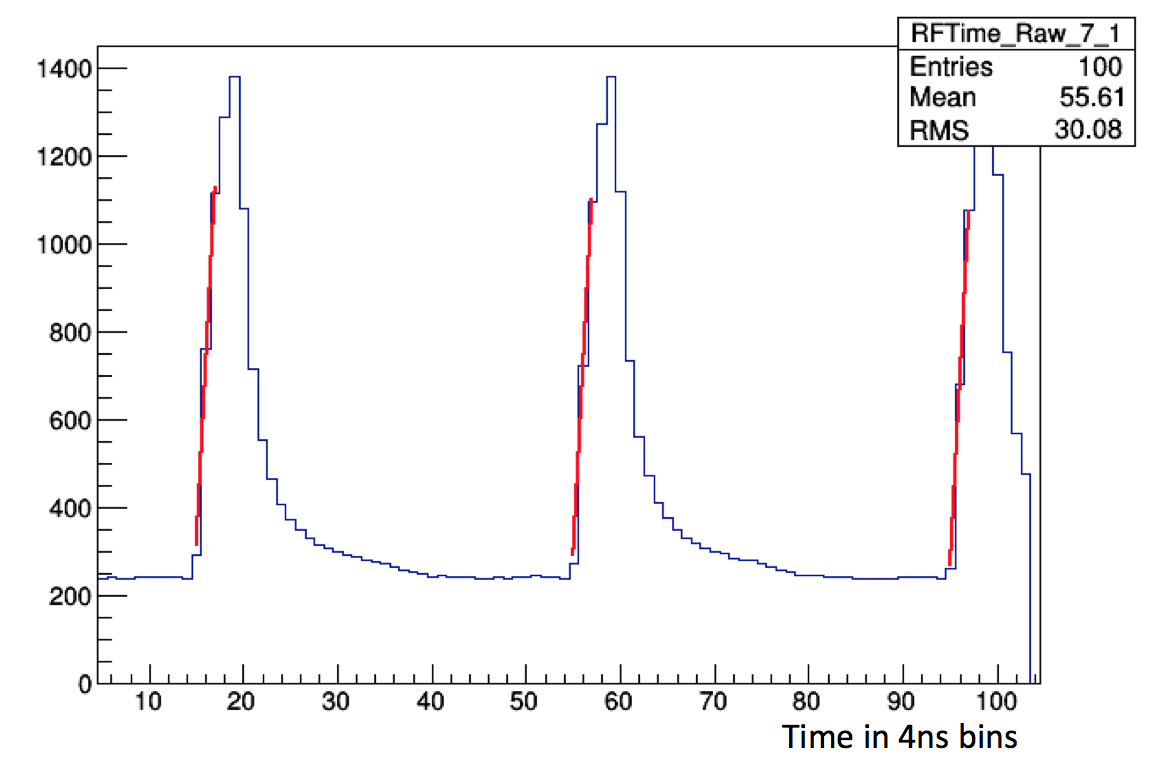
\includegraphics[width=0.7\textwidth]{pics/performance/rfFits.png}
  \caption[Fitted, raw waveform of the RF signal in HPS]{The raw distribution of the RF signal is shown with a straight line fit to the leading edge of the signal.}
  \label{Figure:rfFits}
\end{figure}

The strategy to read off the time from the RF signal was chosen in order to minimize the measured intrinsic resolution of the FADC modules. After identifying the peak bin (4~ns per bin), the pedestal was calculated by averaging the values in 4 bins occurring at 6 to 9 samples prior to the peak. The threshold used in selecting the fitting points was found by calculating the 1/3 height between the averaged pedestal and the peak. The points for the straight line fit were then chosen as the last point below this threshold and the next two points above the threshold. These points were chosen due to the linear uniformity of the pulse away from the
peak bin. The time that was used from this fit was at the half height between the pedestal and the peak. This combination of parameters minimized the width of the time difference distribution between the two independently recorded RF signals as shown in Figure~\ref{Figure:intrTres}. 

\begin{figure}[htb]
  \centering
      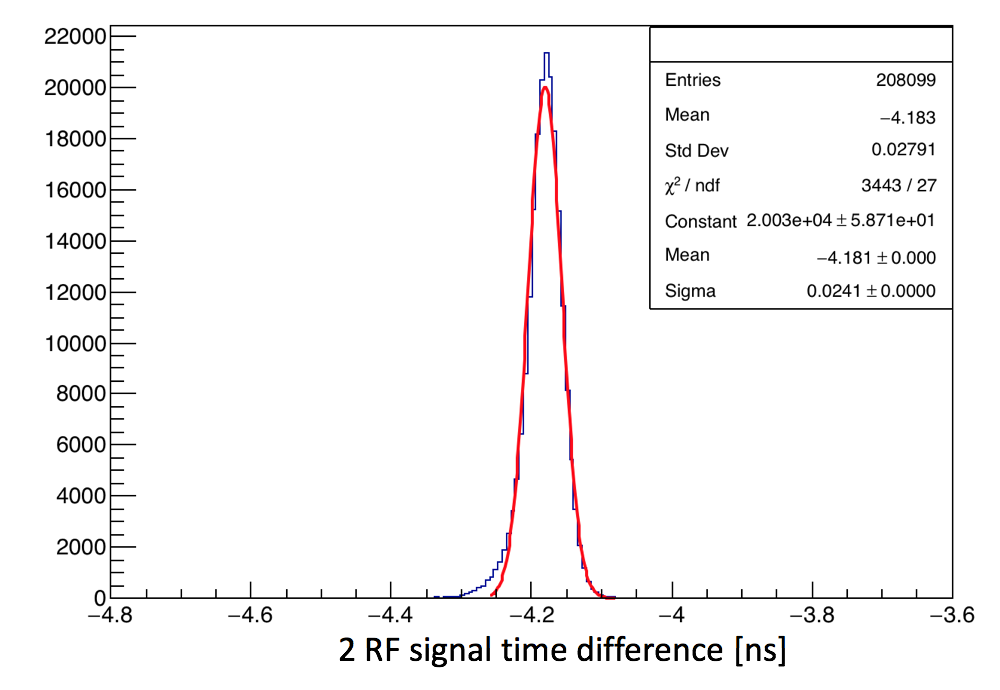
\includegraphics[width=0.7\textwidth]{pics/performance/rfRes.png}
  \caption[FADC intrinsic time resolution]{The intrinsic time resolution of the FADC modules can be obtained by the width of the two RF signal time difference to be approximately 24~ps.}
  \label{Figure:intrTres}
\end{figure}

The internal time resolution of the FADC modules was measured to be approximately 24~ps from the width of the time difference between the two RF signals. We then used the RF signal to precisely calibrate the time offsets of each crystal as follows. The individual crystal module time offsets are measured with respect to the accelerator RF time. For time offsets less than 2~ns, or the time between electron bunches from the accelerator, we calculate the fine time offset per crystal \\

\begin{equation}
	\label{eq:tfine}
	\Delta t_{fine} = \textrm{mod}(t_0 - t_{RF} + N\times 2.004, 2.004) - 1.002 \textrm{ ns}
\end{equation}
where $t_0$ is the time for the crystal as reported from pulse-fitting, $t_{RF}$ is the RF time, and $N$ is an arbitrarily large integer to shift the distribution to all positive values. 2.004~ns is the period of the 499~MHz accelerator RF frequency. Before applying Equation~\eqref{eq:tfine}, we observe the beam bunch structure in the time difference between the crystal hits and the RF time in Figure~\ref{Figure:beamBunch}. 

\begin{figure}[htb]
  \centering
      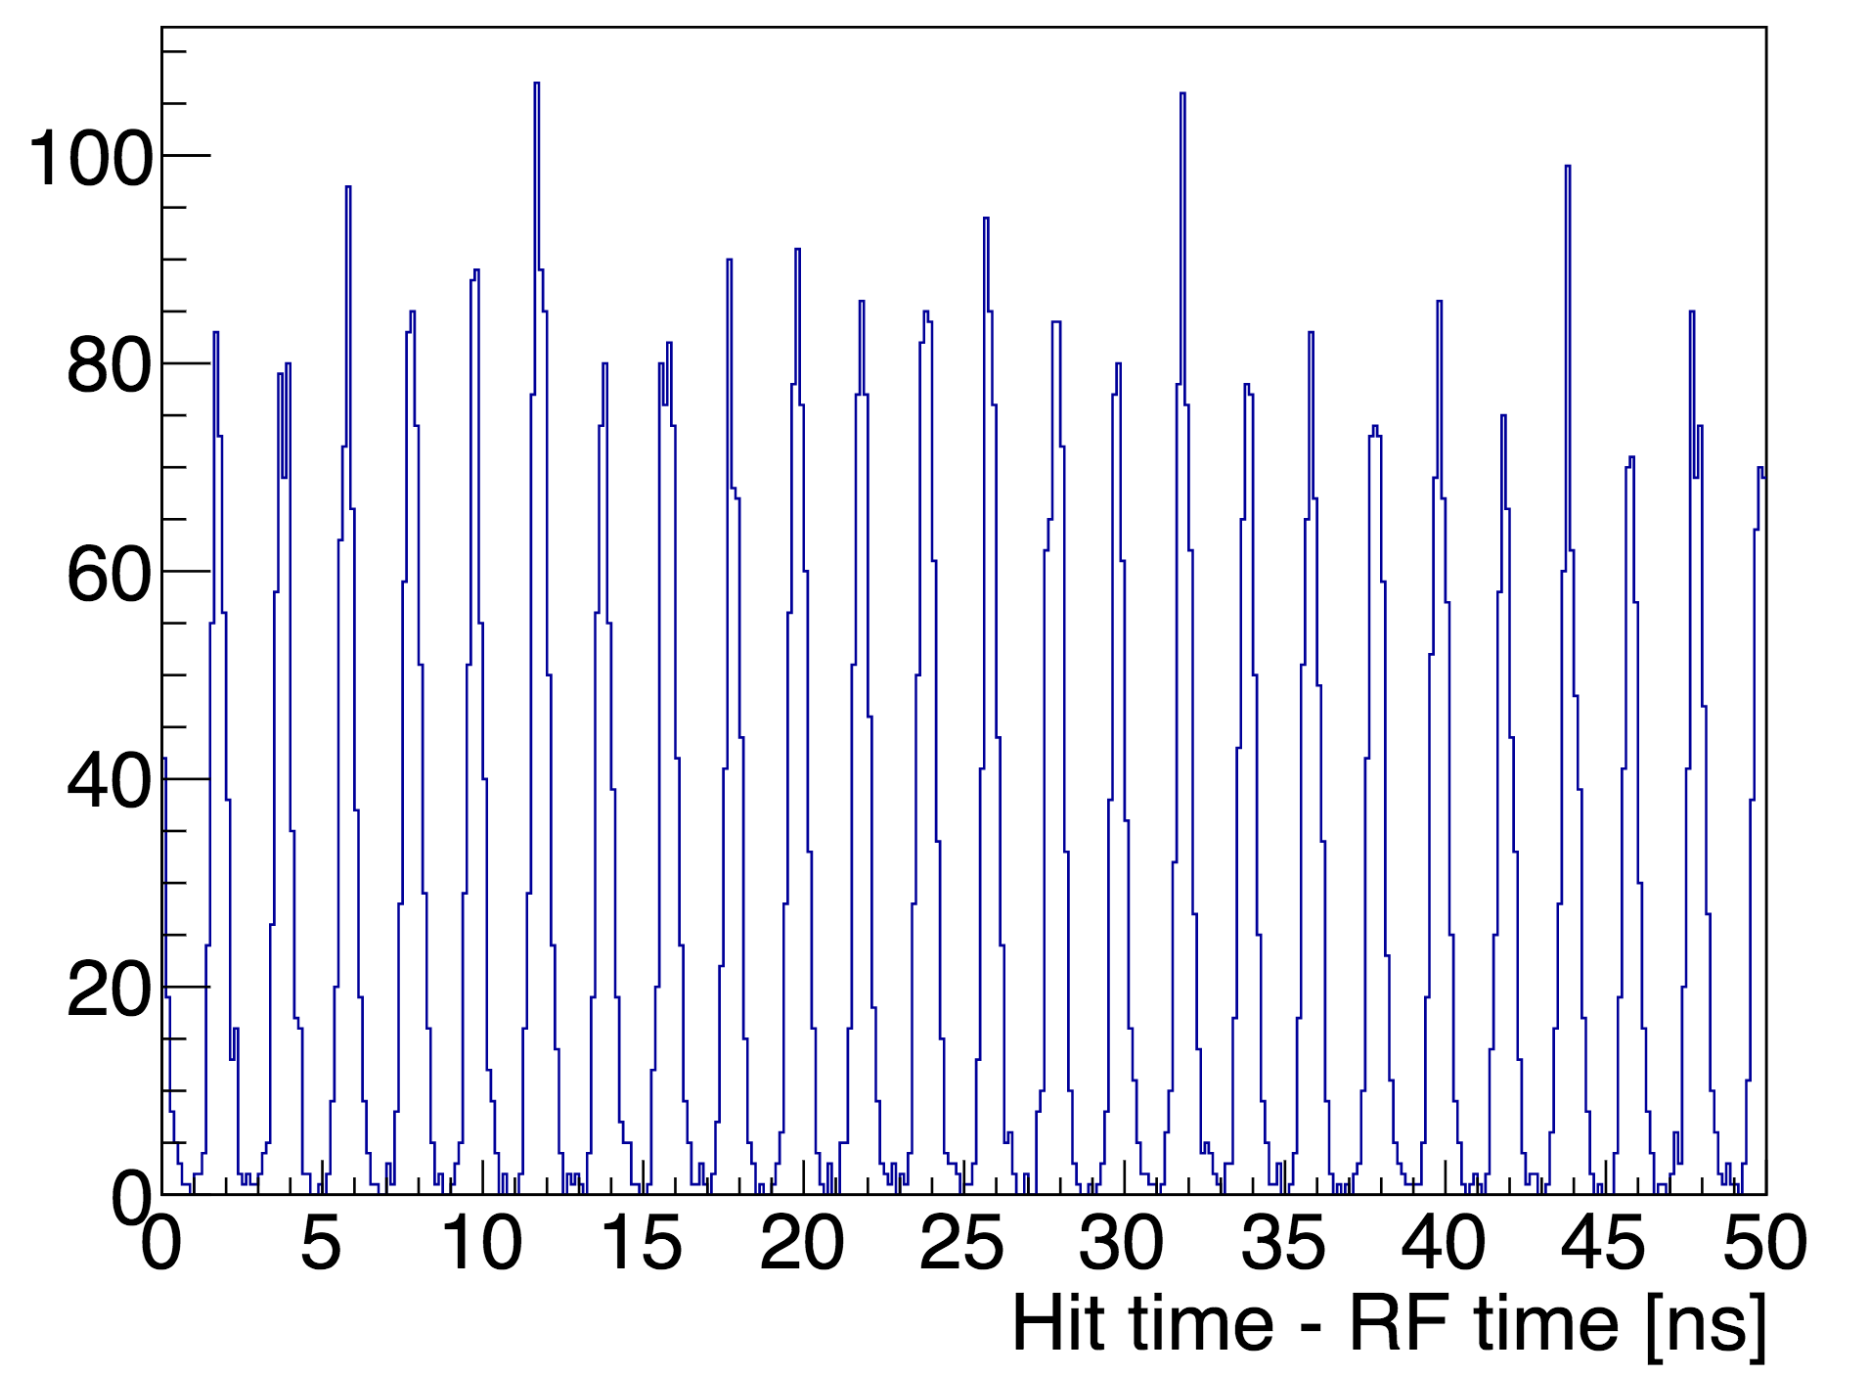
\includegraphics[width=0.7\textwidth]{pics/performance/beamStructure.png}
  \caption[Time difference between ECal hits and RF time]{The time difference between ECal hits and the RF time showing the electron beam bunch structure of approximately 2~ns, consistent with the known accelerator frequency.}
  \label{Figure:beamBunch}
\end{figure}
By applying Equation~\eqref{eq:tfine} to the data of Figure~\ref{Figure:beamBunch}, we can align all of the signals and see the fine offset of each module with respect to the RF time. This technique only shows the offset component that is less than 2~ns and results in all crystals being aligned to the nearest 2$n$~ns, where $n$ is an integer.\\ 
\indent To fully align the crystals, we choose a crystal to align with the RF signal at 0, and then align all other crystals with respect to this crystal. Because the primary trigger for HPS is a cluster pairs trigger, we can compare the time difference between clusters to make this correction. The time of the highest energy hit in a cluster was used to set the time for the cluster. Comparison studies exploring the use of an energy-weighted cluster time using the hit times in a cluster found no significant difference due to the seed hit energy dominating the time distribution and produced the same results as if one had used the time from the seed hit only. Well-correlated pairs of clusters were selected by looking for pairs with an energy sum equal to the beam energy and an energy difference of less than 200~MeV. The times for both clusters must have occurred in the 30--70~ns time window for the 2015 engineering run. The time difference correction between pairs of clusters after the fine time offset correction is shown in Figure~\ref{Figure:2clusoffset}.

\begin{figure}[htb]
  \centering
      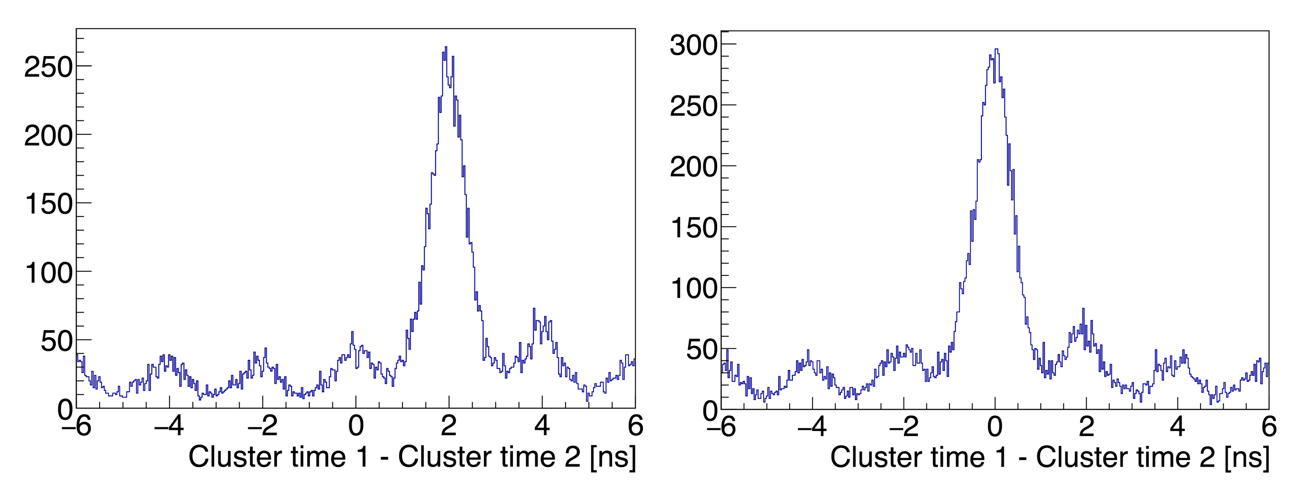
\includegraphics[width=0.9\textwidth]{pics/performance/2clusteroffset.png}
  \caption[Time difference between two clusters after fine offset time correction]{A histogram of the difference in cluster times for two-cluster events after correcting all clusters with the fine timing offset correction. Clusters are aligned to the nearest 2~ns time offset with respect to the RF signal. Shown on the left is a cluster pair that has an overall 2~ns time difference that needs to be corrected for. The plot on the right shows a different cluster pair with an offset centered at 0.}
  \label{Figure:2clusoffset}
\end{figure}

In Figure~\ref{Figure:2clusoffset}, a 2~ns offset between a cluster pair is seen on the left prior to this step in the timing correction with respect to the RF signal. A different cluster pair, shown on the right, has no overall time offset. \\
\indent After correcting for the time offsets of all crystals with respect to the RF time, an energy-dependent correction, known as the time walk correction, must be accounted for. Time walk is the time difference of different amplitude signals crossing threshold in an ADC due to the finite rise time of the leading edge. The effect causes lower energy particles to cross the threshold later in time than higher energy particles. This effect can be removed by studying the time difference between a cluster hit and the seed hit as a function of the cluster hit energy. Pulse fitting of the raw signal removes most of the time walk when compared to other methods that can be used to obtain a hit time. In the 2015 engineering run data, the seed hit was greater than 400 MeV and provided a reasonable threshold against which to compare hit times at lower energies. For the 2016 engineering run data, the time walk correction was able to use a much higher seed hit threshold of 1~GeV, and the energy-dependence could be extended to higher energies. The time walk can be extracted from the comparison of the hit times within a cluster as shown in Figure~\ref{Figure:hittimeincluster}.

\begin{figure}[htb]
  \centering
      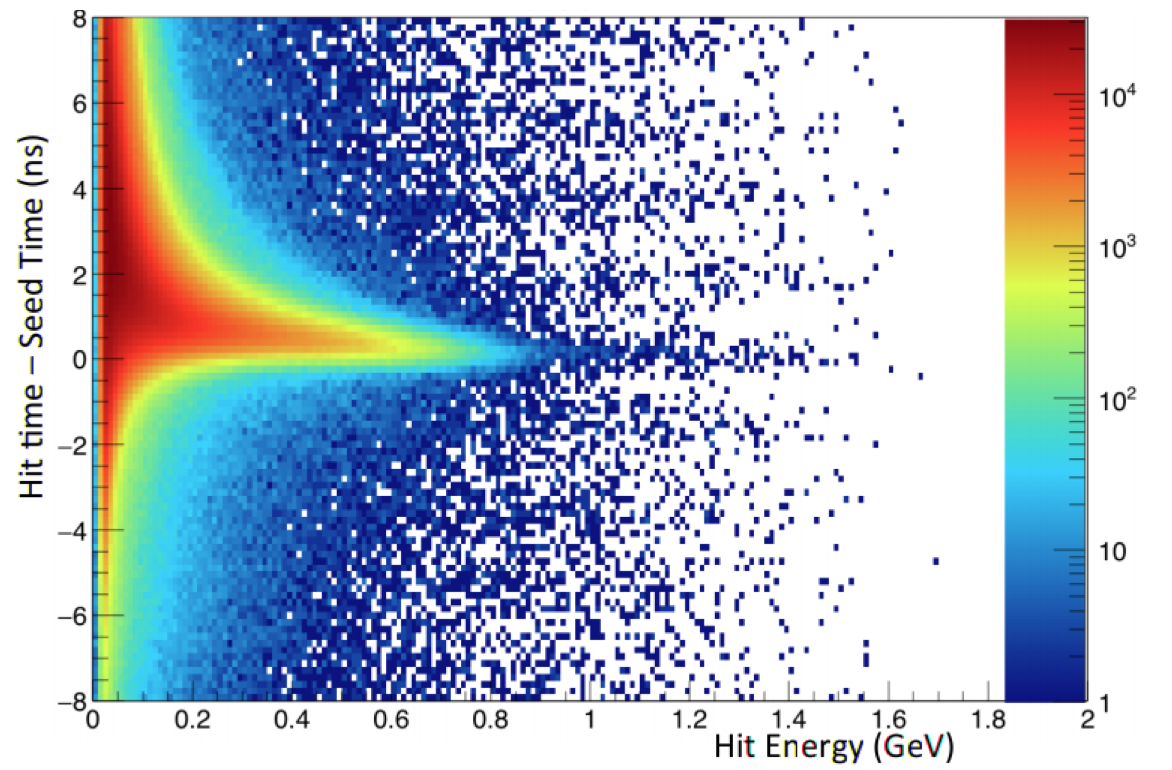
\includegraphics[width=0.7\textwidth]{pics/performance/hittimeincluster.png}
  \caption[Hit times in a cluster versus the hit energy]{The time walk correction for the 2016 data can be extracted from the time difference between each cluster hit time versus the seed hit time plotted versus the hit energy.}
  \label{Figure:hittimeincluster}
\end{figure}

The time walk correction found from the 2016 engineering run data is shown in Figure~\ref{Figure:twalk} and is described by:
\begin{figure}[htb]
  \centering
      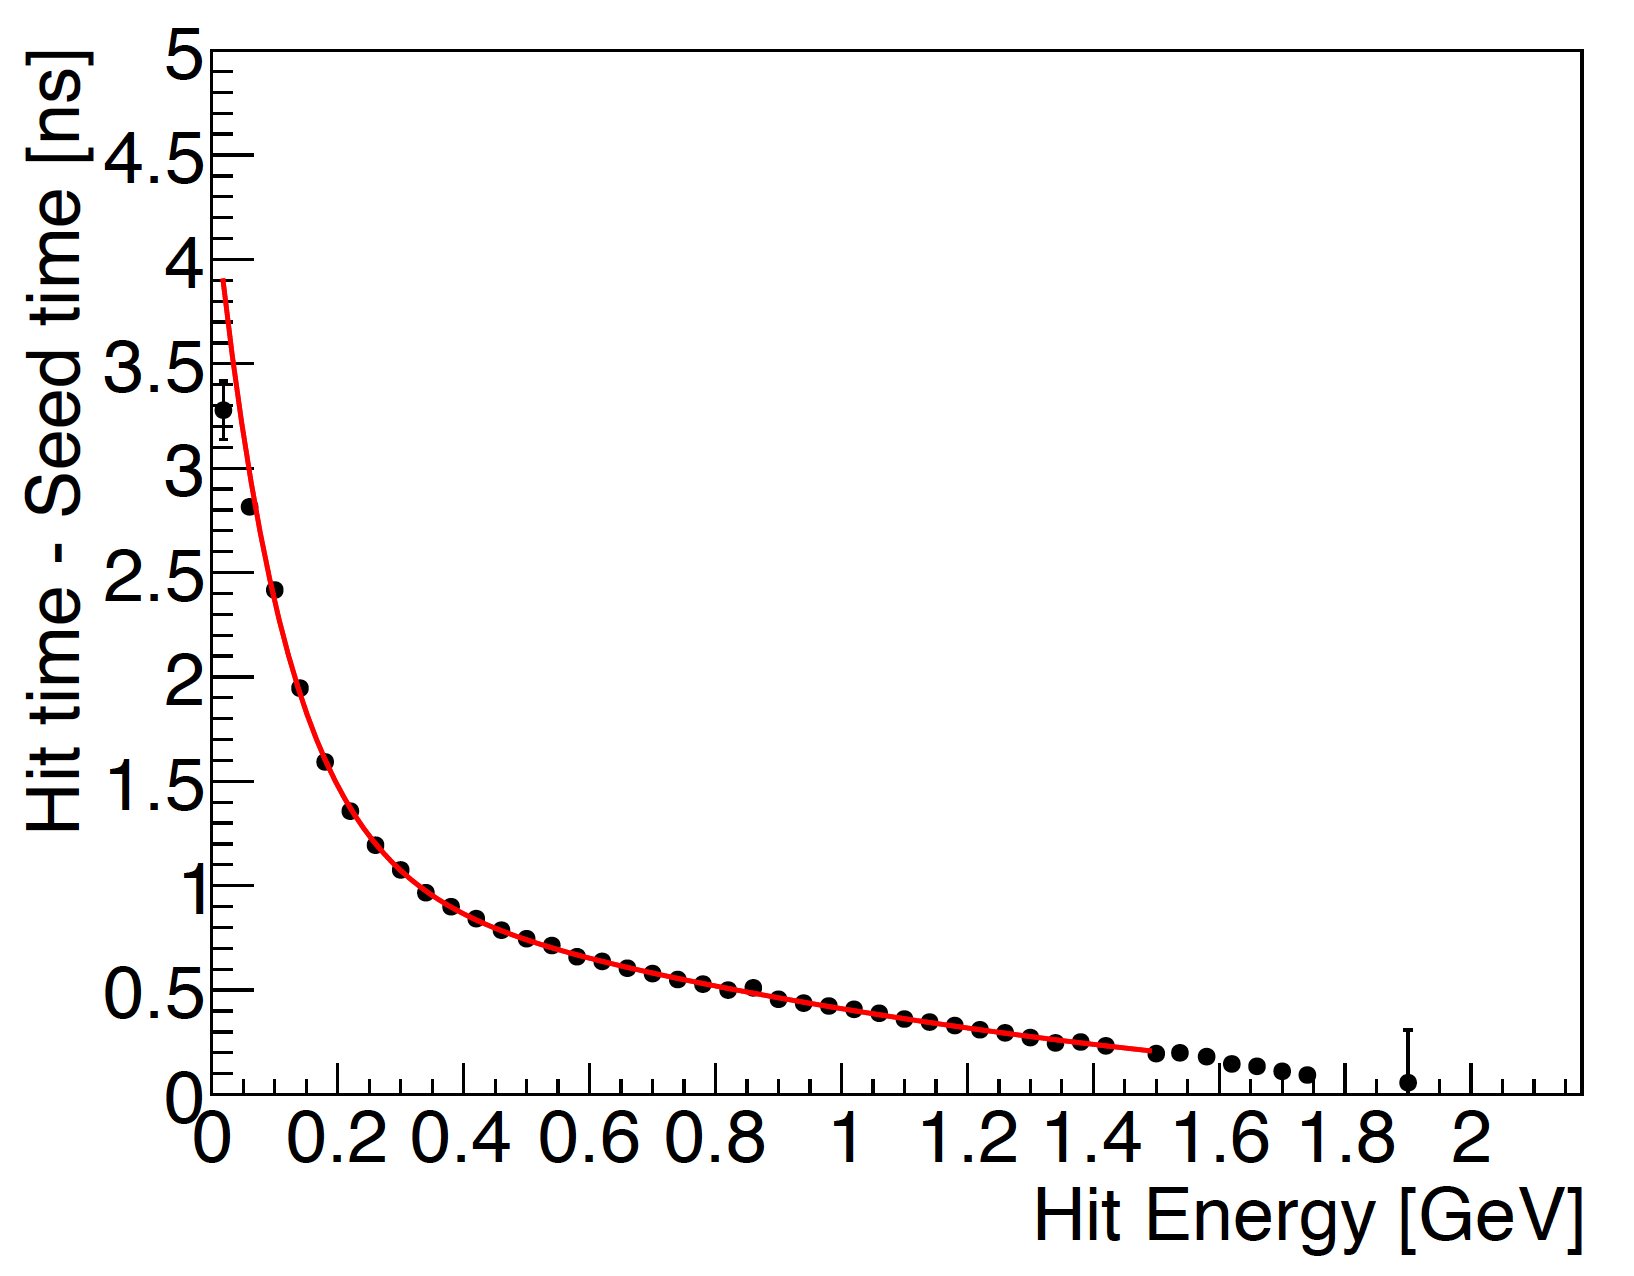
\includegraphics[width=0.6\textwidth]{pics/performance/twalk2016.png}
  \caption[Time walk correction for the 2016 engineering run ECal data]{The time walk correction for the 2016 engineering run data was found by plotting the time difference between each cluster hit time and the seed hit time versus the crystal hit energy.}
  \label{Figure:twalk}
\end{figure}
\begin{equation}
	\label{eq:twalkEq}
		\Delta_{t_{walk}} = e^{p_0+p_1E}+p_2+p_3E+p_4E^2	
\end{equation}
After removing all crystal-to-crystal time offsets and applying the energy-dependent time walk correction to all modules, the resulting time resolution for all energies is shown in Figure~\ref{Figure:timeRes} and described by:
\begin{figure}[htb]
  \centering
      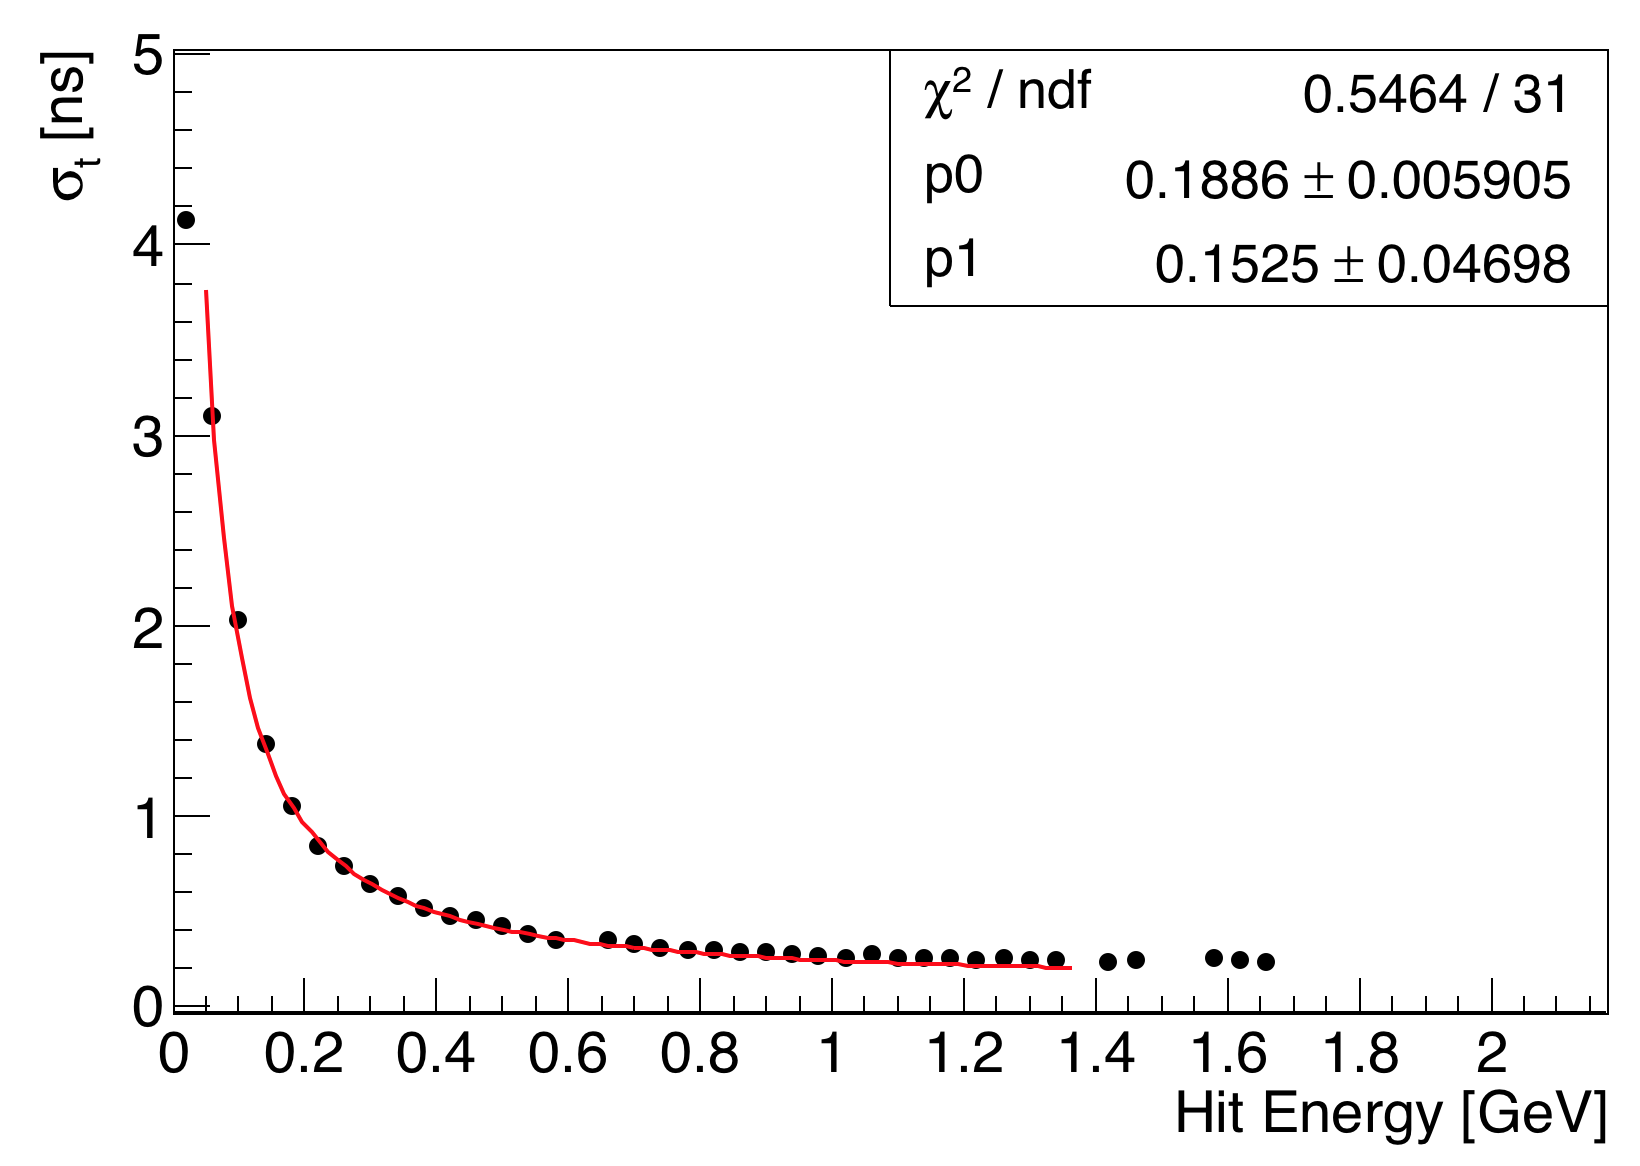
\includegraphics[width=0.6\textwidth]{pics/performance/timeRes2016.png}
  \caption[Time resolution of the ECal for the 2016 run ]{The time resolution as a function of energy.}
  \label{Figure:timeRes}
\end{figure}
\begin{equation}
	\label{eq:twalkEqn}
		\sigma_t \textrm{ [ns]} = \dfrac{p0}{E}\oplus p1	
\end{equation}
The final measured time resolution for the time difference between two clusters is shown in Figure~\ref{Figure:timeRes2cl}.
\begin{figure}[htb]
  \centering
      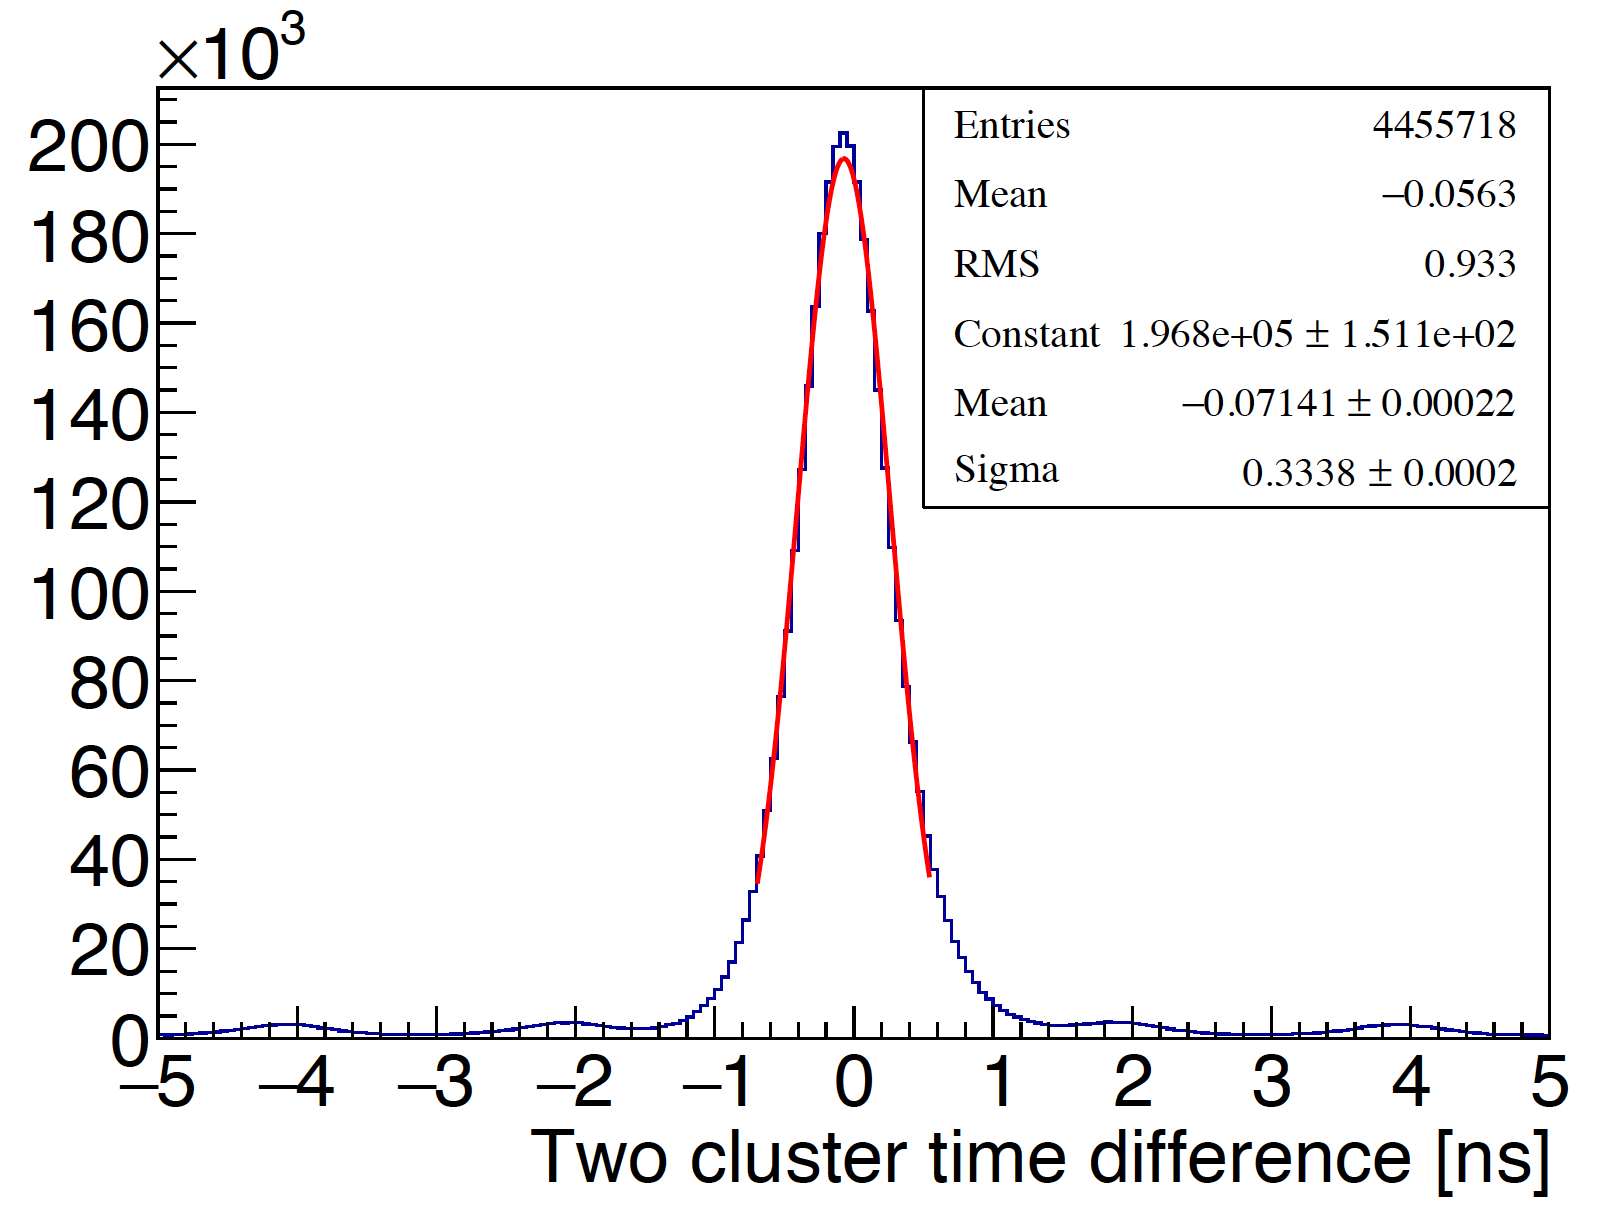
\includegraphics[width=0.6\textwidth]{pics/performance/2clusterTres.png}
  \caption[Time resolution for the time difference between two clusters]{The fully calibrated time difference between two clusters is shown from the 2016 engineering run. The energies sum to greater than 80$\%$ of the beam energy and have a resulting resolution of approximately 330~ps.}
  \label{Figure:timeRes2cl}
\end{figure}
As shown in Figure~\ref{Figure:timeRes2cl}, for two clusters that have an energy sum greater than 80$\%$ of the beam energy in 2016, the resolution is approximately 330~ps. For the 2015 engineering run at a lower beam energy, the resolution of the time difference between two clusters was found to be approximately 470~ps. 

%\subsection{Experimental agreement with Monte Carlo}
%
%After accounting for all backgrounds, the energy sum of the two particles is in general agreement between Monte Carlo and data as shown in Figure~\ref{fig:mcAgree}.
%
%\begin{figure}[htb]
%  \centering
%      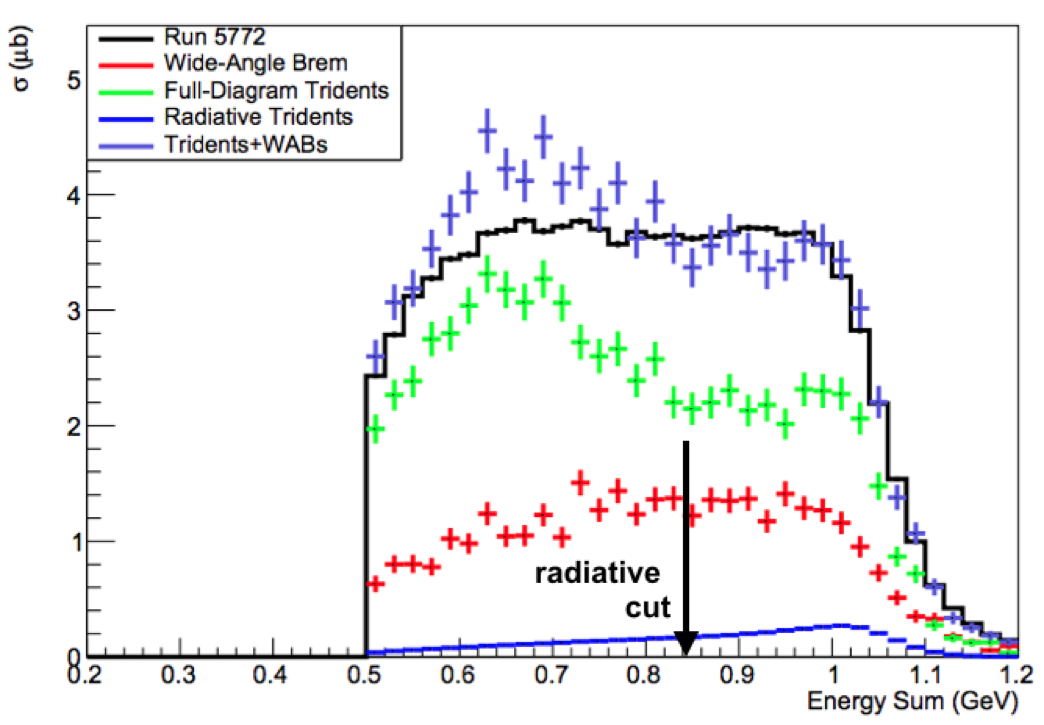
\includegraphics[width=0.8\textwidth]{pics/searching/mcAgree.png}
%  \caption[Energy sum comparison in Monte Carlo and data]{Energy sum in Monte Carlo and data. The energy sum is in general agreement at the high end of the spectrum where HPS is optimized to search for heavy photons. Further studies to isolate track and SVT layer inefficiencies at the lower energy sum are still being explored.}
%  \label{fig:mcAgree}
%\end{figure} 
%
%The agreement between data and Monte Carlo is critical to the HPS experiment for estimating the overall radiative fraction, or fraction of events in the final trident sample that can be attributed to purely radiative production. This value is used to project the expected heavy photon yield in the final samples. While there is good agreement between the background simulation and data above the radiative cut at 80$\%$ of the beam energy, there is still widespread disagreement at the low energy sum. The detector efficiencies are still being studied for inefficiencies that may contribute to this difference at the low energy sum.